\section{Short bodies}
\label{sec:short}

We begin by considering short bodies with $1 \le AR \le 2$, to investigate how a modest increase in $\AR$ modifies the bifurcations scenario and the sequence in which the various modes become unstable compared to the well-known $\AR=1$ case. For these aspect ratios, vortices do not form over the lateral sides of the body and the base-flow dynamics is dominated by the TE vortex shedding. This section complements the analysis by \cite{choi-yang-2014}, which examined the secondary instability of the flow past bodies ranging from a normal flat plate ($\AR \rightarrow 0$) to a square cylinder ($\AR=1$).

\subsection{The base flow}

\begin{figure}
  \centering
  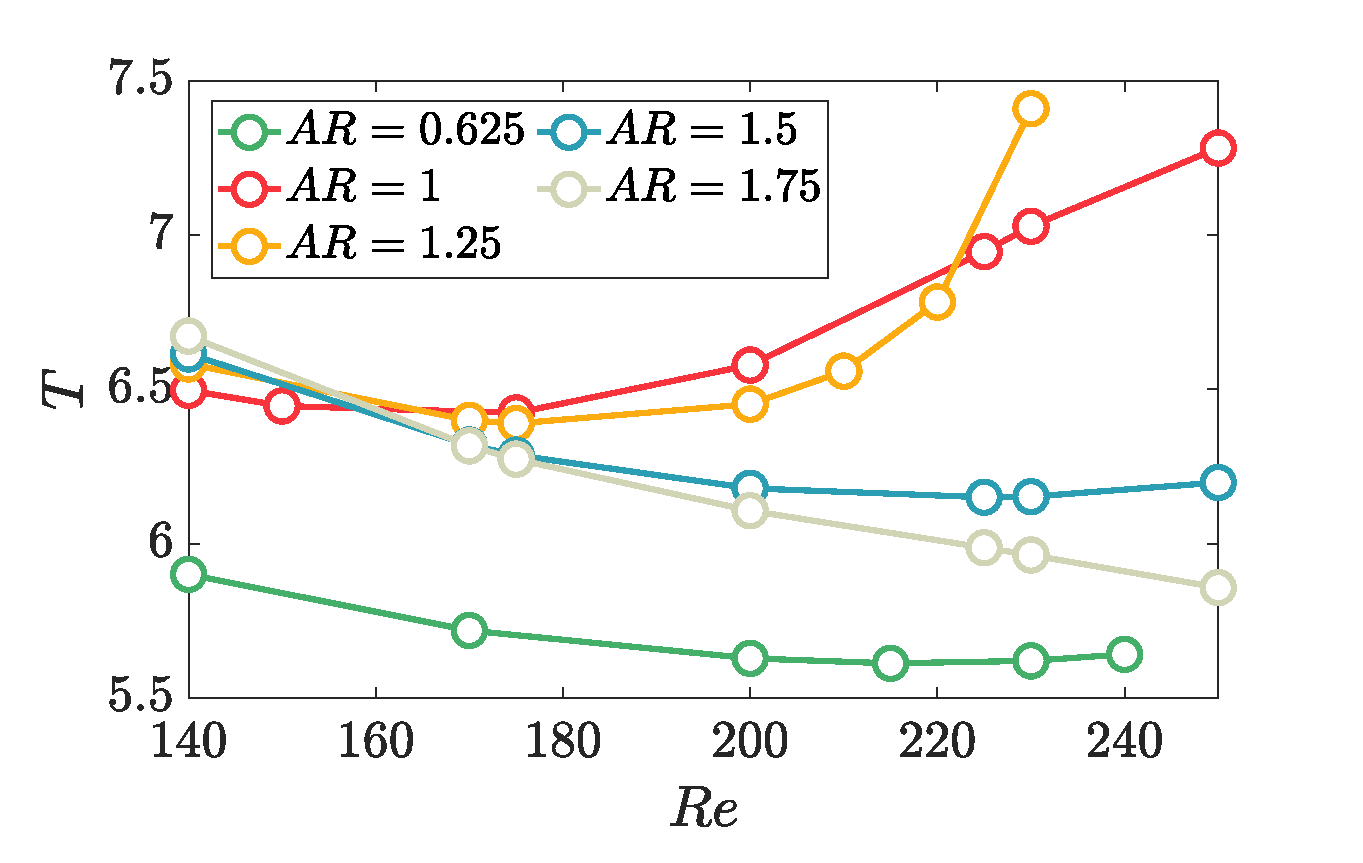
\includegraphics[width=0.49\textwidth]{./fig/AR1s/T_Re.eps}
  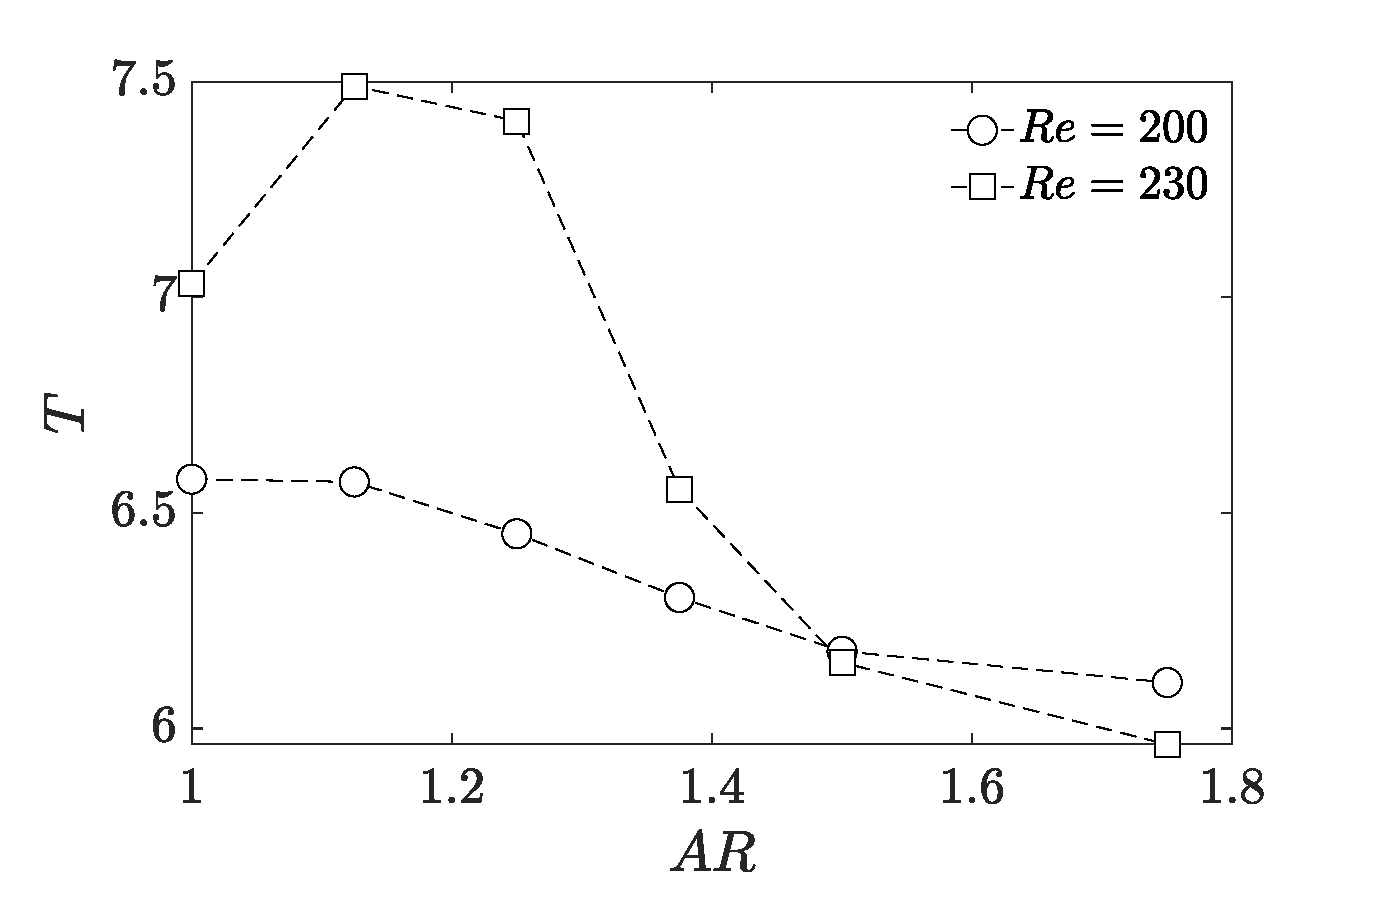
\includegraphics[width=0.49\textwidth]{./fig/AR1s/T_AR.eps}
  \caption{Base-flow period as a function of $\AR$ and $Re$. Left: dependence of $T$ on $Re$ for $1 \le \AR \le 1.75$. Right: dependence of $T$ on $\AR$ for $Re=200$ and $Re=230$.}
  \label{fig:T_Re_small}
\end{figure}
%
We start characterising the influence of $\AR$ and $Re$ on the periodic base flow. Figure \ref{fig:T_Re_small} illustrates the dependence of the base-flow shedding period $T$ on both $Re$ and $\AR$. For the shortes ($\AR \approx 1$) and longest ($\AR \ge 1.5$) bodies, $T$ exhibits mild variations with $Re$: when increasing the Reynolds number from $Re=175$ to $Re=250$ it increases by approximately $11\%$ for $\AR=1$ and decreases by about $7.1\%$ for $\AR=1.75$. In constrast, for intermediate aspect ratios $T$ exhibits a much stronger dependence on $Re$; for $\AR=1.25$, $T$ increases significantly with $Re$ rising from $T \approx 6.4$ at $Re = 175$ to $T \approx 8.3$ at $Re=240$ ($\Delta T = 23\%$). For $\AR=1.25$ we do not report results for $Re > 240$ as at $Re \approx 250$ the 2D base-flow loses its periodicity due to a Neimark-Sacker bifurcation (not shown for brevity). The different dependence of $T$ on $Re$ for the different $\AR$s reflects a variation in the base-flow topology.

\begin{figure}
  \centering
  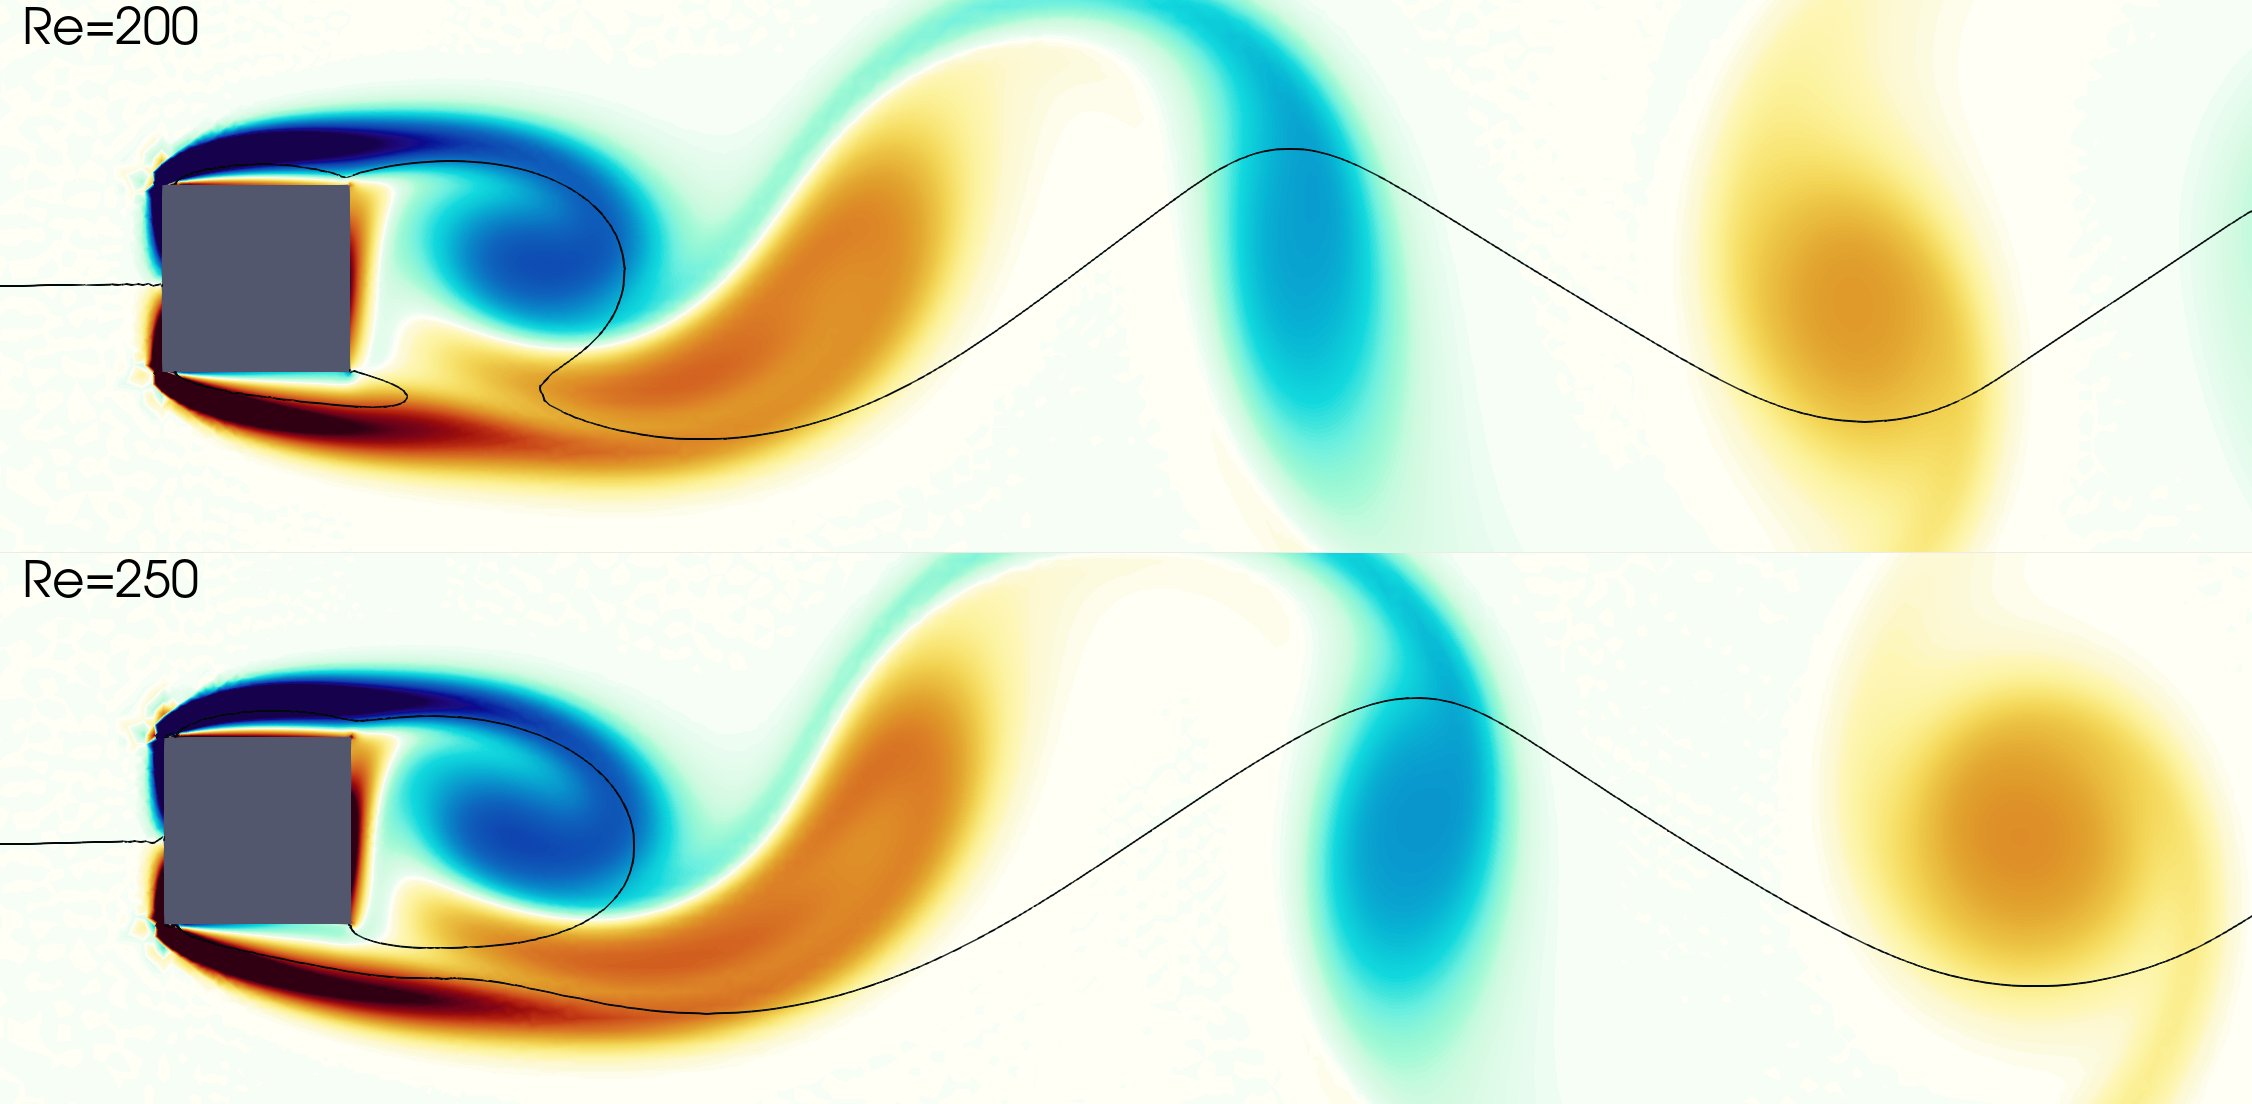
\includegraphics[width=0.49\textwidth]{./fig/AR1/snap/snap.0030.png}
  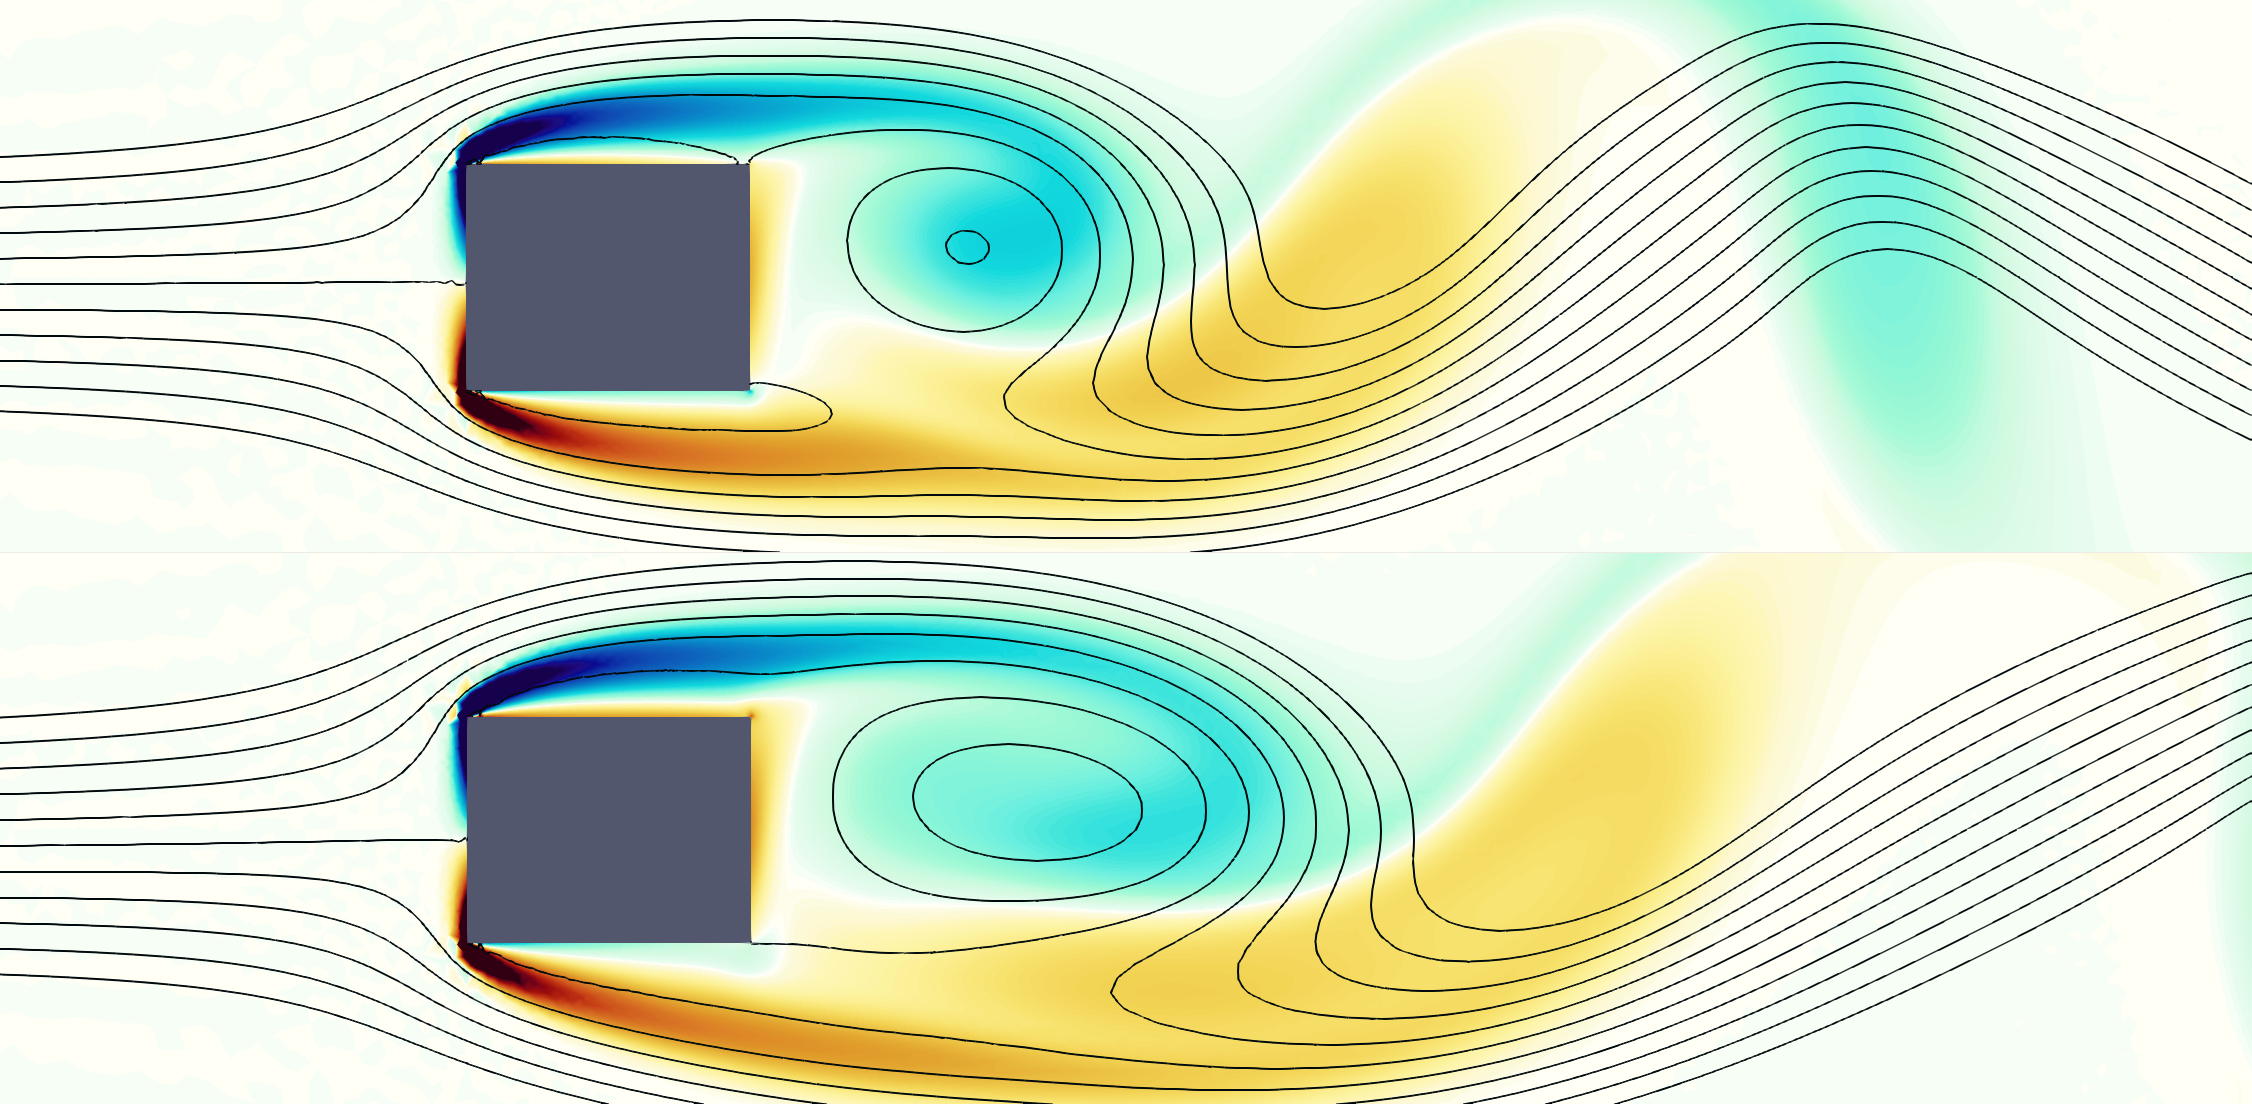
\includegraphics[width=0.49\textwidth]{./fig/AR1p25/snap/snap.0030.png}
  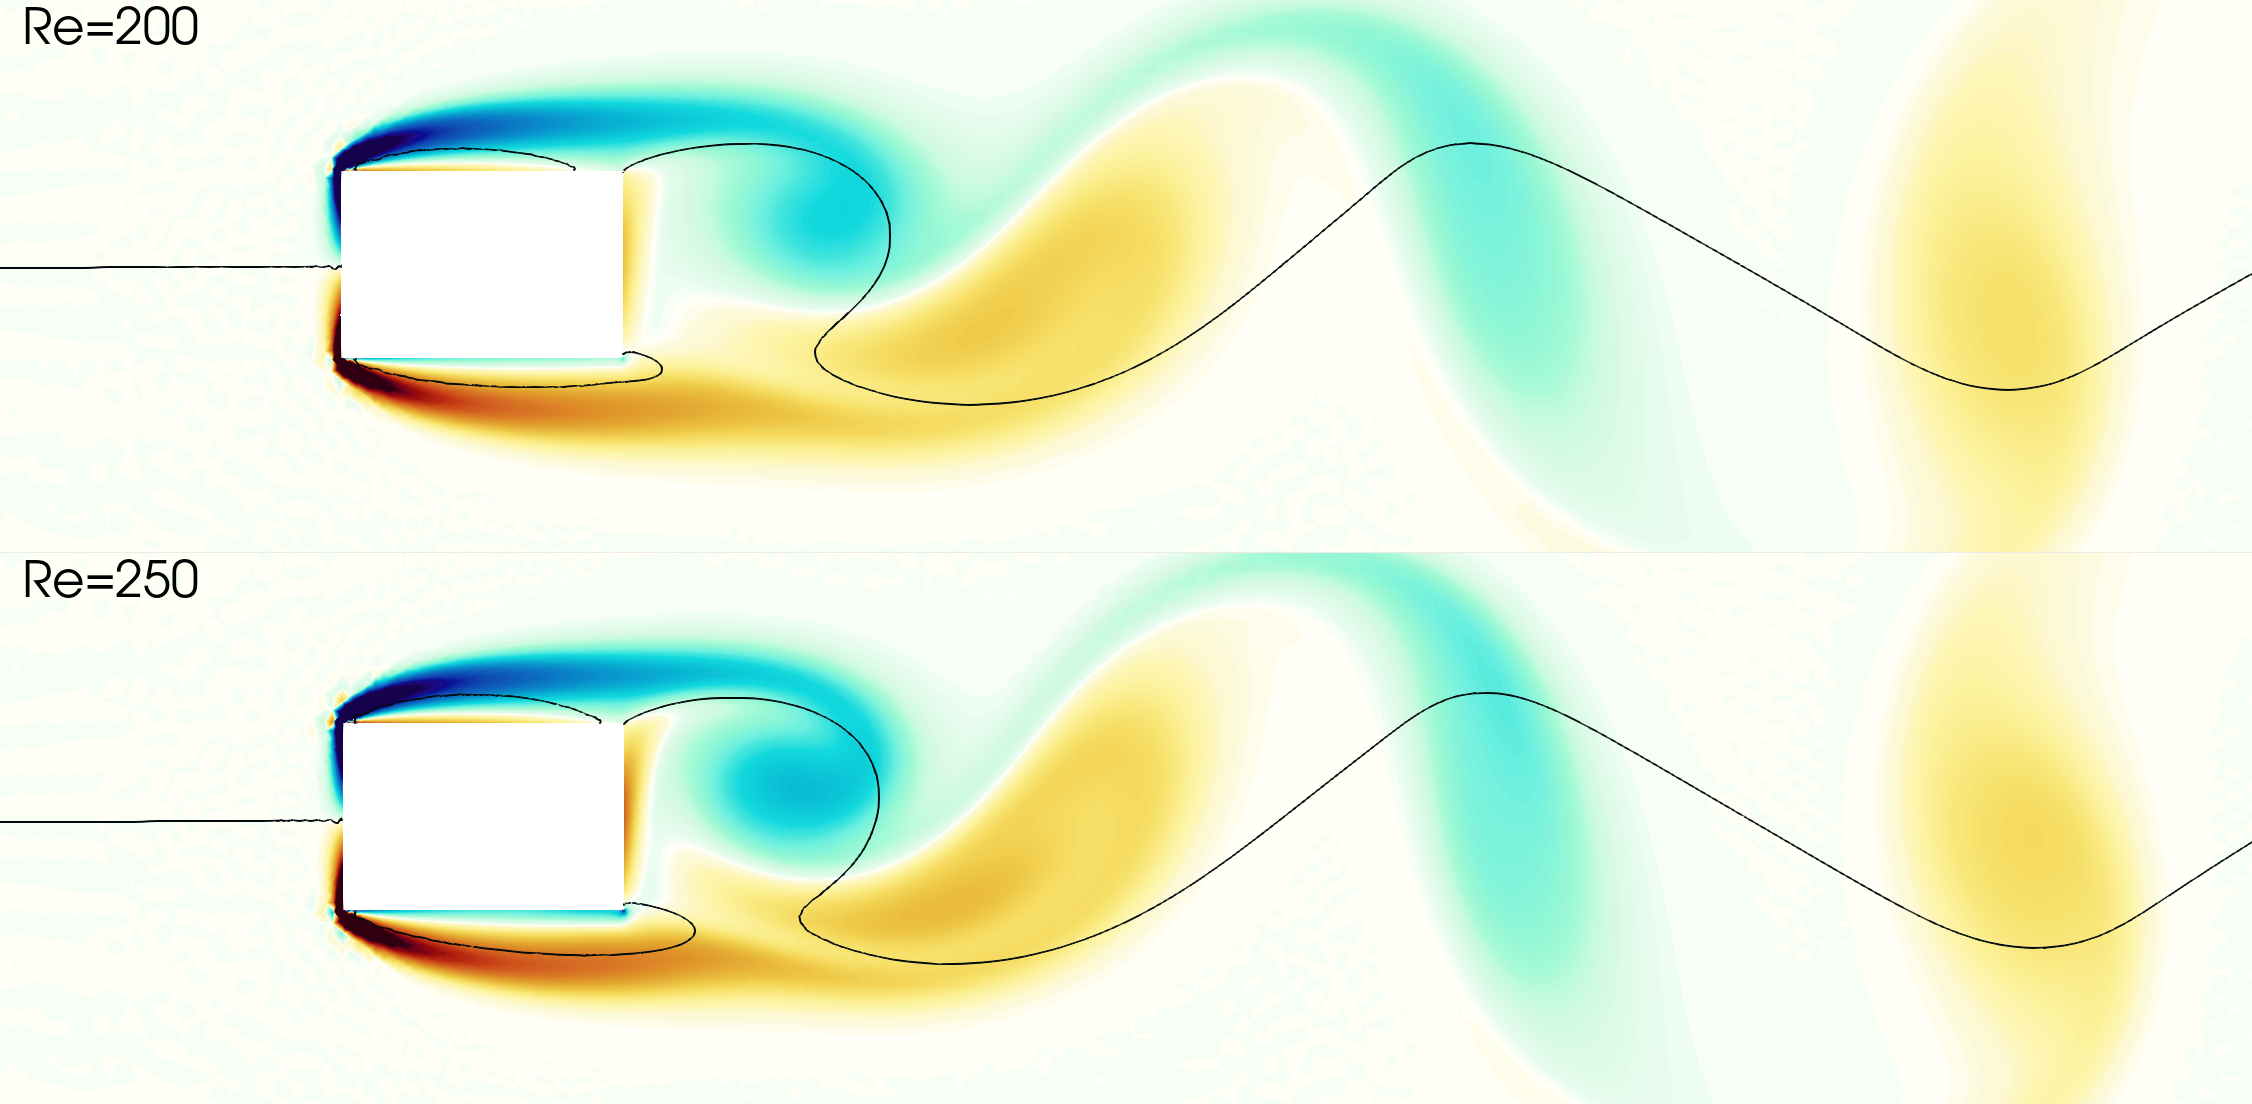
\includegraphics[width=0.49\textwidth]{./fig/AR1p5/snap/snap.0030.png}
  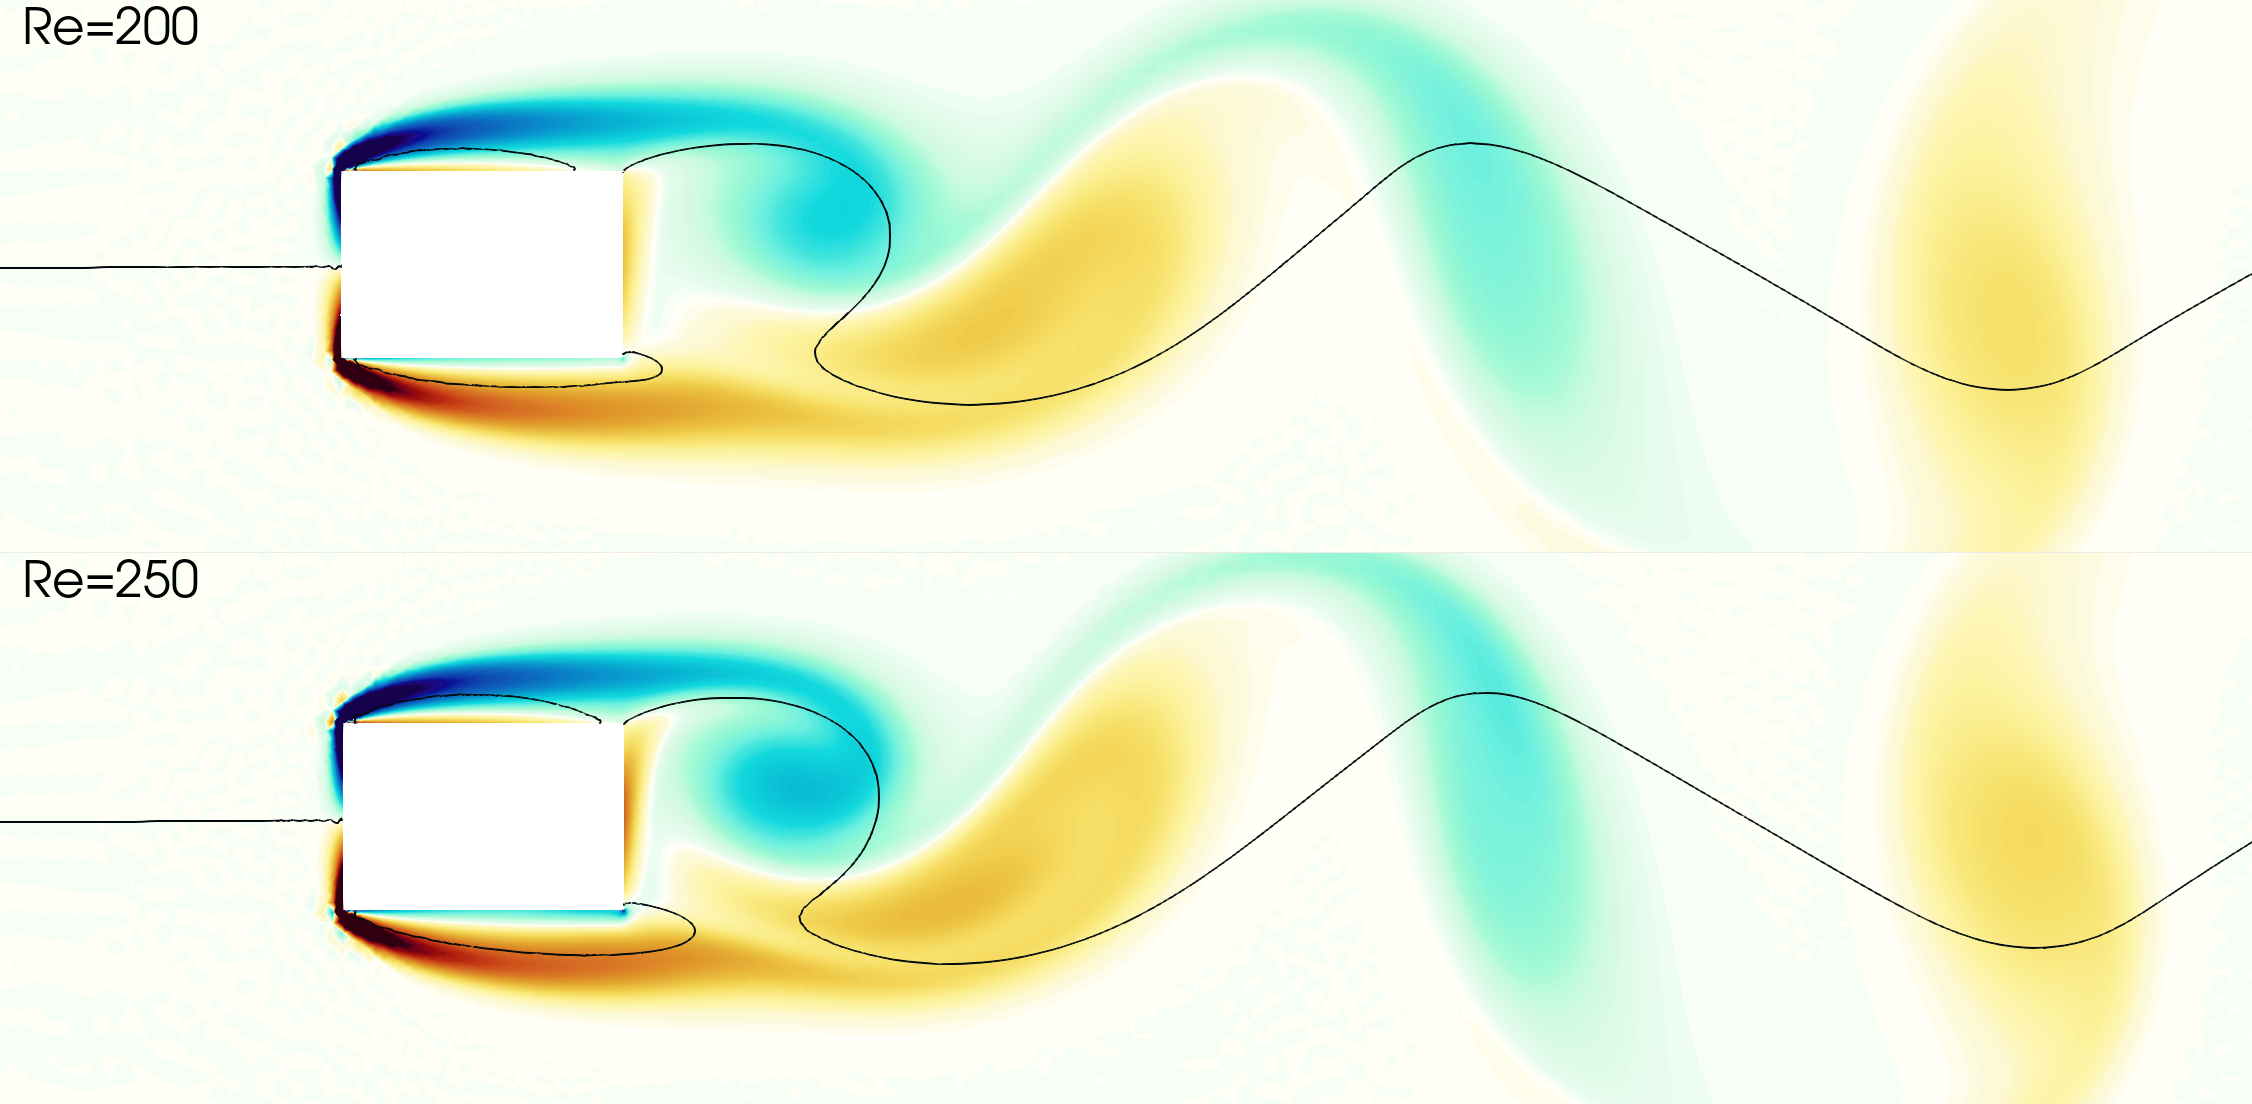
\includegraphics[width=0.49\textwidth]{./fig/AR1p5/snap/snap.0030.png}  
  \caption{Instantaneous snapshots of the base-flow vorticity for $\AR=1$ (top left), $\AR=1.25$ (top right), $\AR=1.5$ (bottom left) and $\AR=1.75$ (bottom right) at $Re=200$ (top) and $Re=250$ (bottom). For all cases the snapshots are taken at the same phase, i.e. just before the shedding of a vortex with negative vorticity in the wake. XX REPLACE $\AR=1.75$ AND ORGANISE THE FIGURE FROM TOP TO BOTTOMXX}
  \label{fig:bf-short}
\end{figure}
%
The influence of $\AR$ on the base-flow topology is shown in figure \ref{fig:bf-short}. For the smaller $\AR < 1.25$, for all considered $Re$ the flow separates at the LE and only rarely reattaches along the lateral sides of the body. In this case the vortex shedding in the wake is thus determined by the dynamics of the LE shear which is indeed active in the formation of the wake vortex. This is visualised in the figure \ref{fig:bf-short} by the streamline separating from the LE that indeed delimits the wake vortex before it is shed in the wake. By contrast, for the larger $\AR>1.25$the LE shear layer (intermittently) reattaches along the lateral sides of the body at all $Re$, and the wake dynamics is mostly determined by the TE shear layer.
For the intermediate $\AR=1.25$ the base-flow topology changes with $Re$. At the lower $Re \le 210$ the flow resembles what has been observed for longer bodies (with the LE shear layer intermittently reattaching along the lateral sides of the body), and the wake vortex shedding is driven by the TE shear layers. At the higher Reynolds numbers ($Re>210$), instead, the flow recovers the low-$\AR$ topology, with the wake dynamics being primarily driven by the LE shear layers. This is visualised in figure \ref{}, when comparing panels xx and xx and noting that the streamline separating at the LE corner reattaches for $Re=200$, but not for $Re=250$. This change of topology is explained with the fact that an increase of $Re$ leads to an increase of the angle with which the flow separates at the LE corners.

\begin{figure}
  \centering
  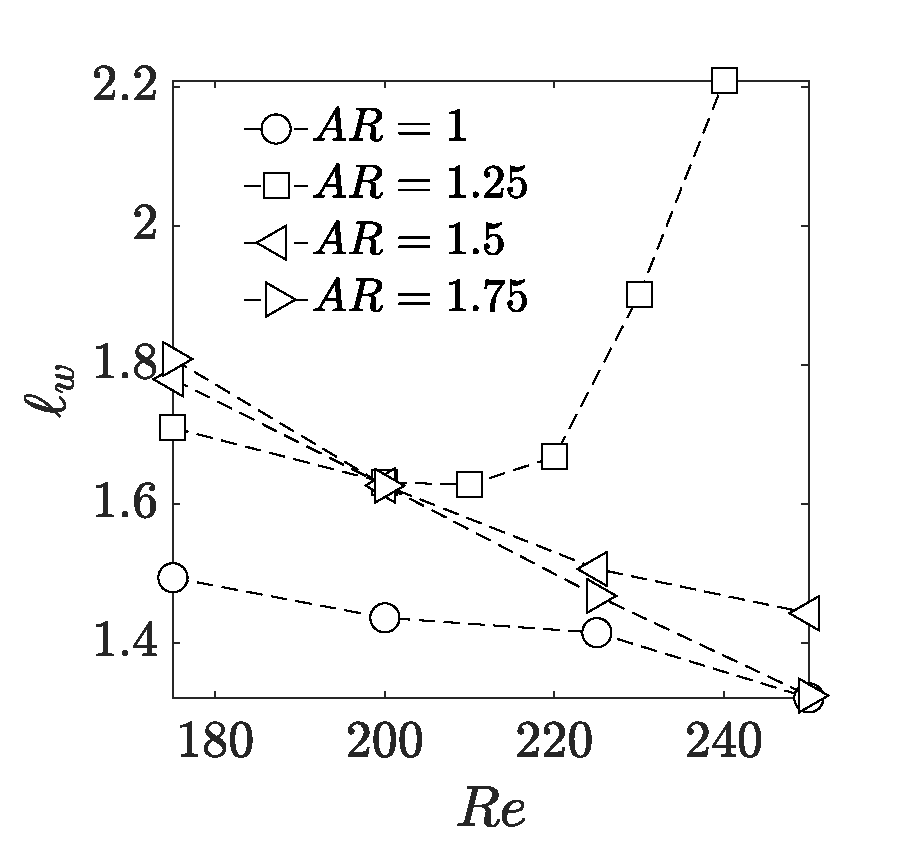
\includegraphics[width=0.32\textwidth]{./fig/AR1s/lw.eps}
  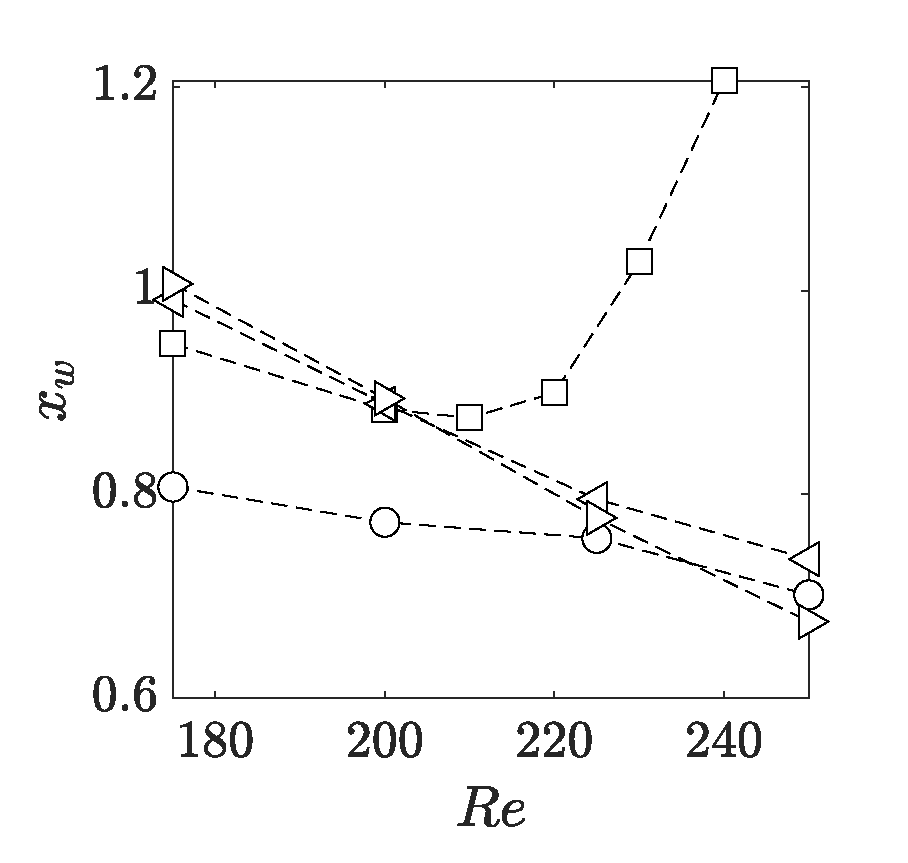
\includegraphics[width=0.32\textwidth]{./fig/AR1s/xw.eps}
  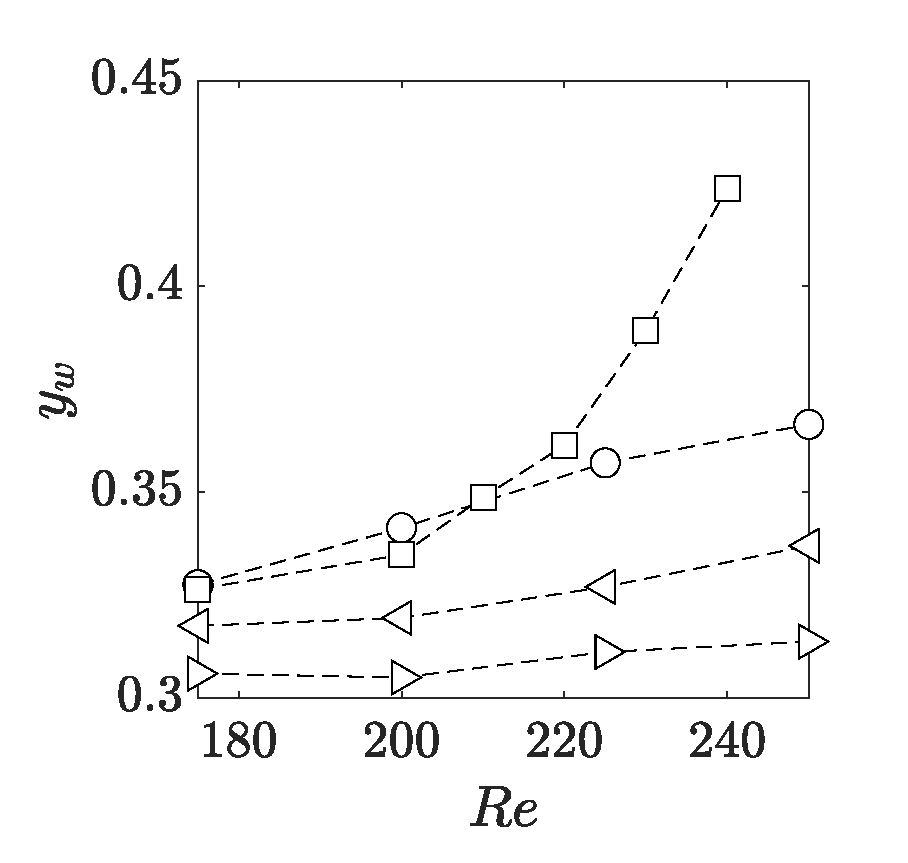
\includegraphics[width=0.32\textwidth]{./fig/AR1s/yw.eps}
  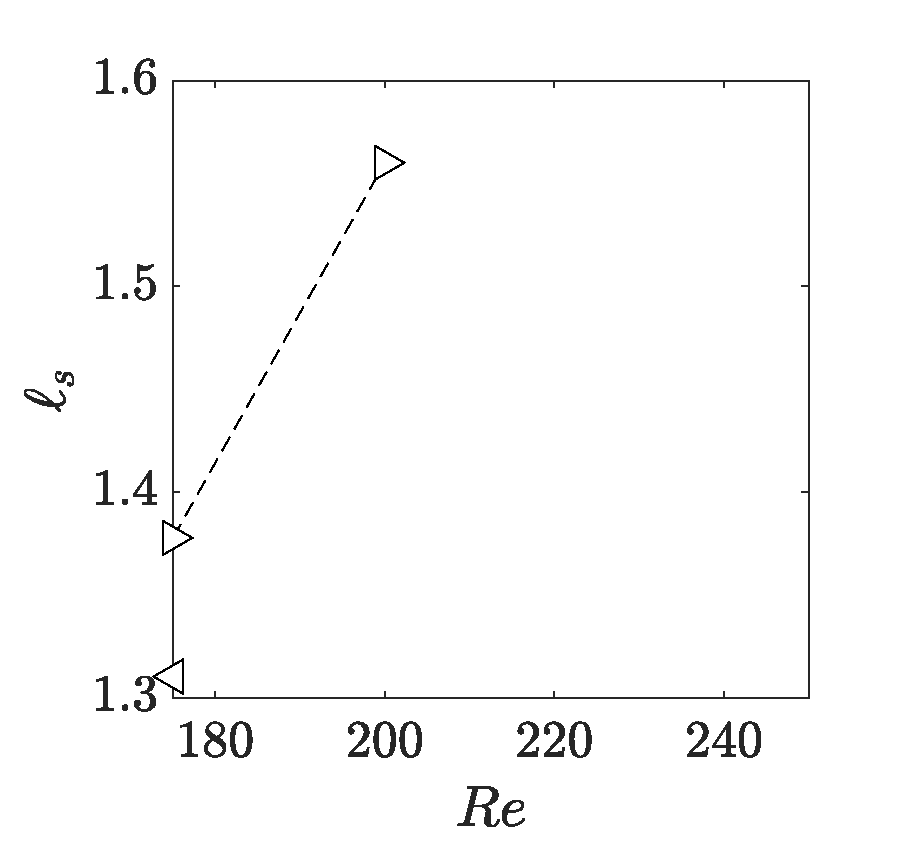
\includegraphics[width=0.32\textwidth]{./fig/AR1s/ls.eps}
  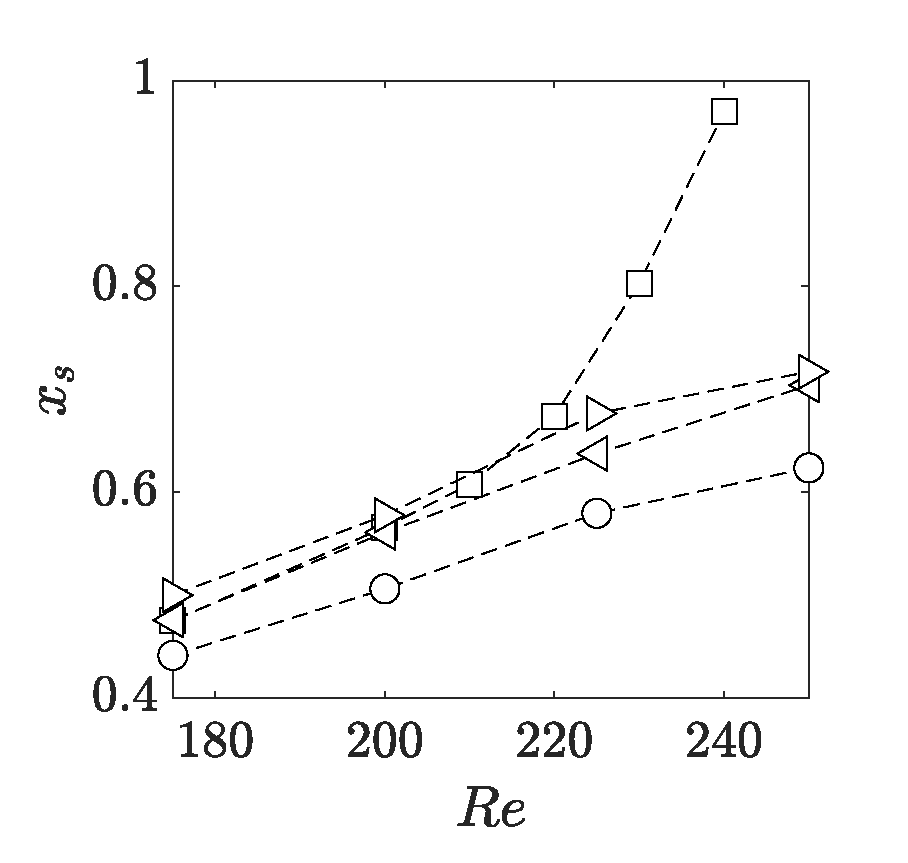
\includegraphics[width=0.32\textwidth]{./fig/AR1s/xs.eps}
  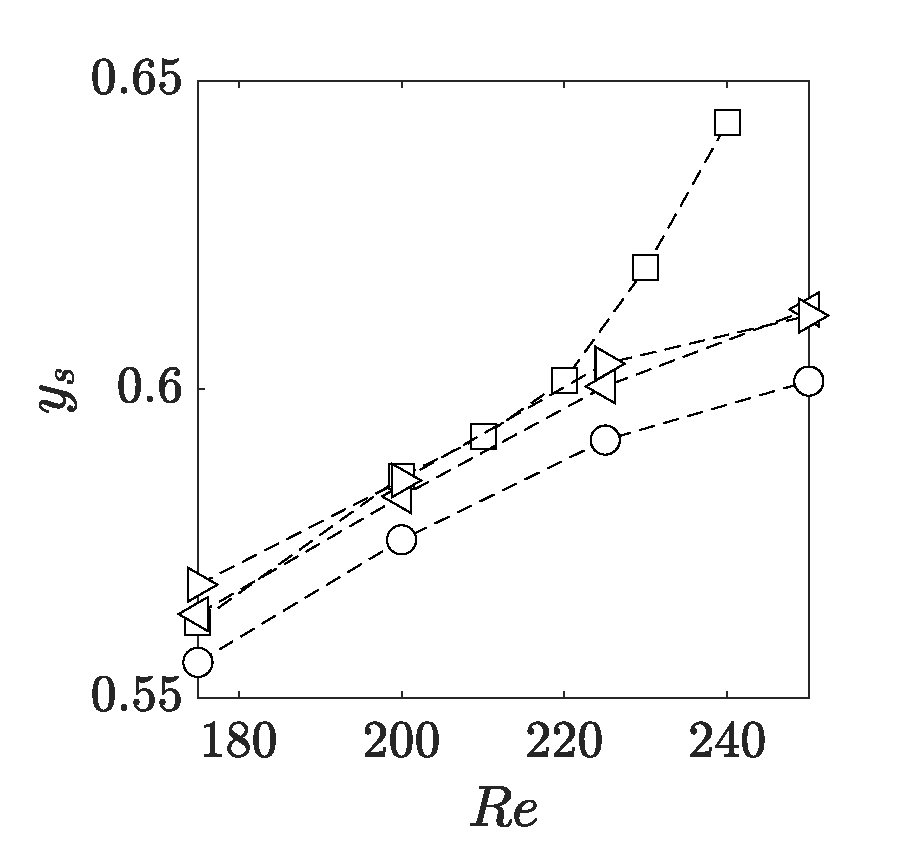
\includegraphics[width=0.32\textwidth]{./fig/AR1s/ys.eps}
  \caption{Dependence of the mean-flow properties on $\AR$ and $Re$ for $1 \le \AR \le 1.75$ and $175 \le Re \le 250$.}
  \label{fig:mf_lengths}
\end{figure}
%
We look at the mean flow averaged over one shedding period; see figure \ref{fig:mf_lengths}. For all $\AR$ an increase of $Re$ leads to an increase of the angle with which the flow separates; see dependence on $Re$ of $y_s$ and $y_w$. As a result the LE shear layers become thicker as $Re$ increases, being thus responsible for the decrease of $\ell_w$. For $\AR=1.25$ the an increase of the Reynolds number leads to a fast increase of $\ell_w$ (and $x_w$) for $Re>210$, which well correlates with the increase of the shedding period. Note that, on average, the flow reattaches along the lateral sides of the body only for $\AR \ge 1.5$ and $Re \le 200$.
% 
\begin{figure}
  \centering
  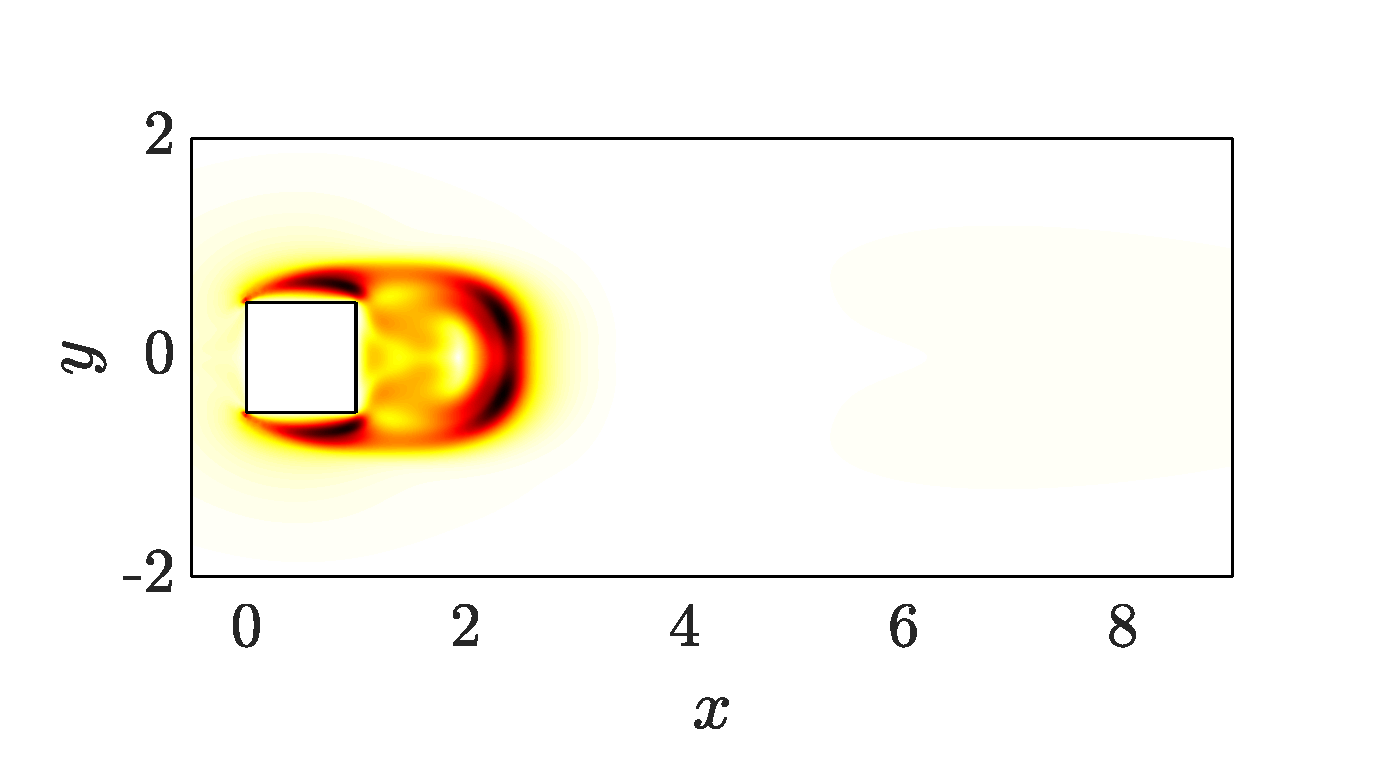
\includegraphics[width=0.49\textwidth]{./fig/AR1/LinStab/sens_Re250.eps}
  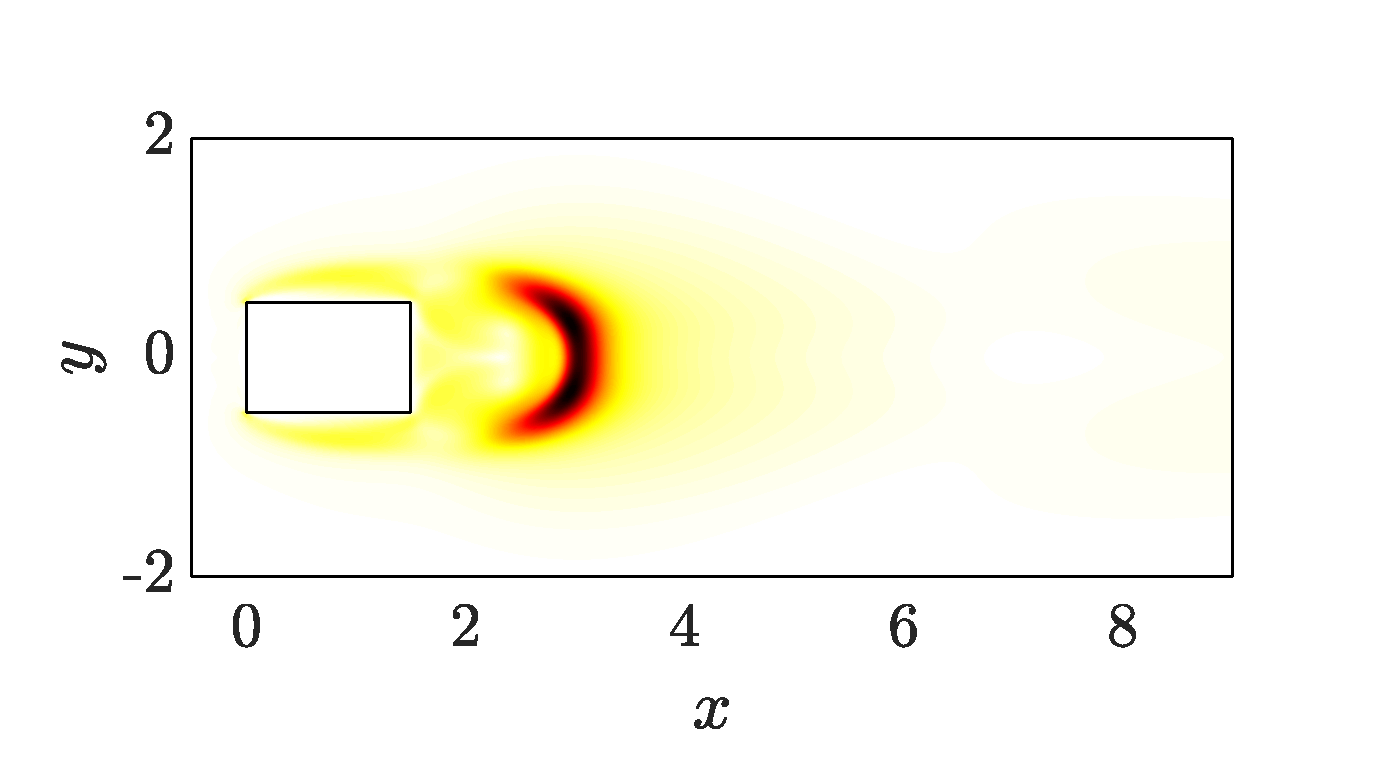
\includegraphics[width=0.49\textwidth]{./fig/AR1p5/LinStab/sens_Re250.eps}
  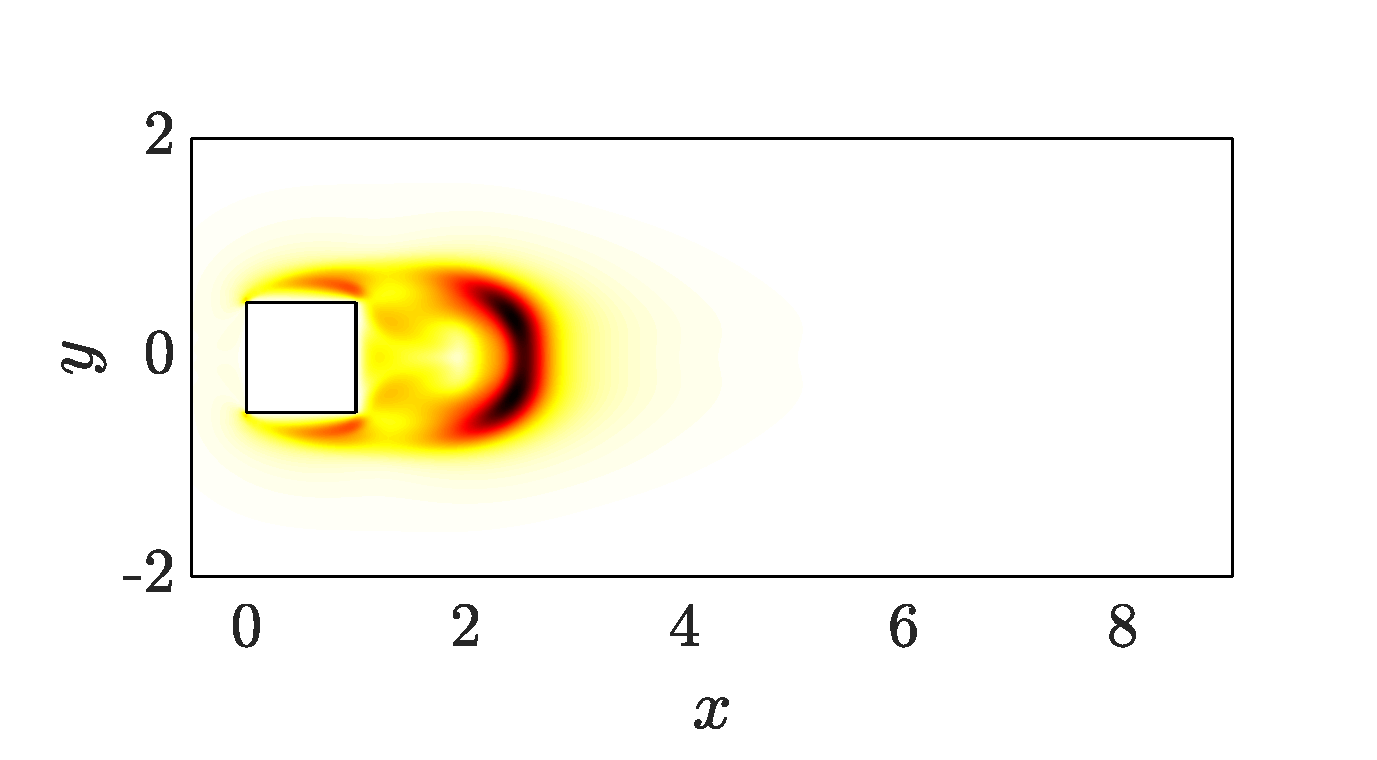
\includegraphics[width=0.49\textwidth]{./fig/AR1p25/LinStab/sens_Re200.eps}
  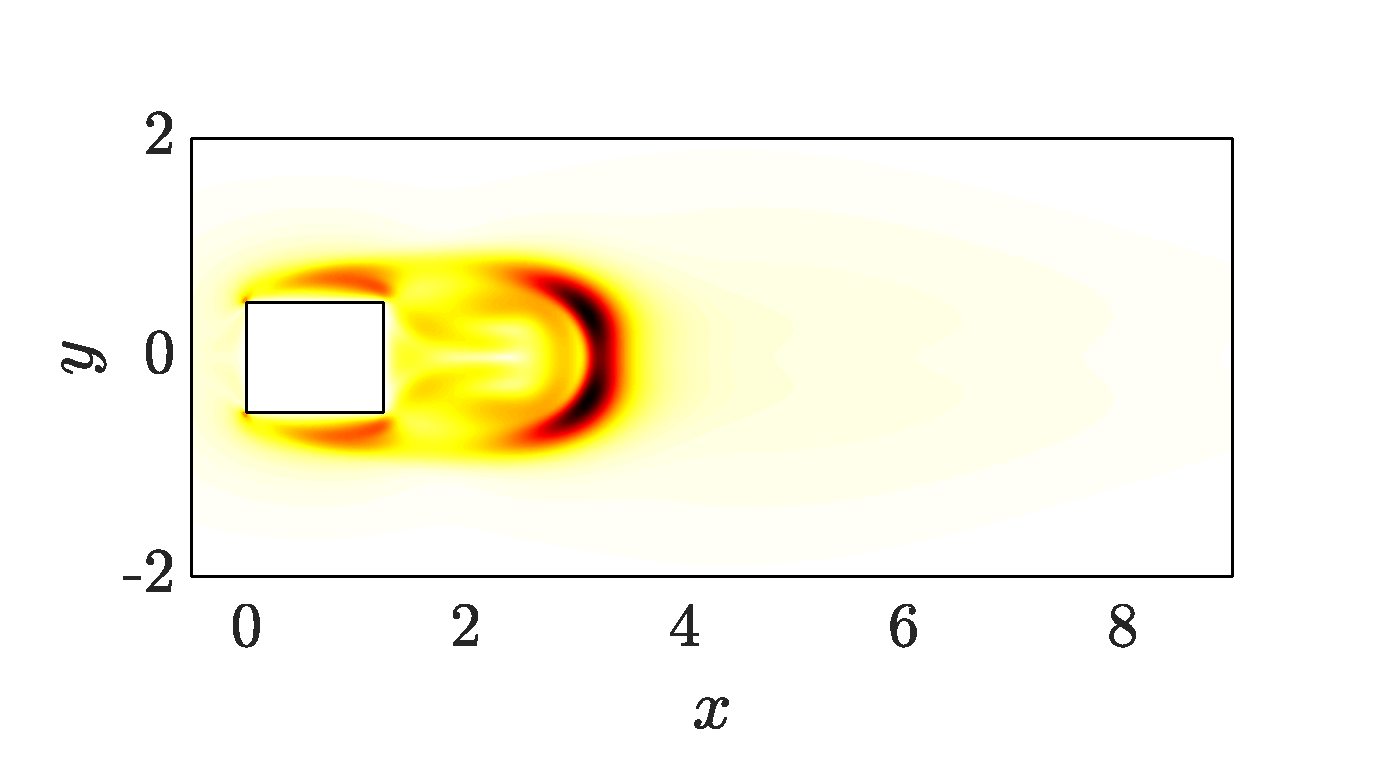
\includegraphics[width=0.49\textwidth]{./fig/AR1p25/LinStab/sens_Re230.eps}
  \caption{Linear stability analysis of the mean fow for $\AR=1$ and $Re=250$ (top left), $\AR=1.5$ and $Re=250$ (top right), $\AR=1.25$ and $Re=200$ (bottom left) and $\AR=1.25$ and $Re=230$ (bottom right).}
  \label{fig:mf_sens}
\end{figure}
%
To further highlight the change of the flow topology with $\AR$ and $Re$, we perform a global stability analysis of the mean flow averaged over one shedding period. The focus in on the leading eigenmode, which is representative of the unsteady phenomena of the flow. For a similar approach see for example \cite{pier-2002,barkley-2006} for the circular cylinder and \cite{chiarini-quadrio-auteri-2022} for rectangular cylinders. 
%
The frequency of the leading eigenmode predicts fairly well the Strouhal number observed in the nonlinear simulations for all cases, with a maximum difference of $xx\%$. Unlike the case of the circular cylinder, which is marignally stably \citep{barkley-2006}, the present mean flow stability analysis leads to a slightly negative growth rate. Figure \ref{fig:mf_sens}, shows the structural sensitivity of the leading mode. The structural sensitivity was introduced by \cite{giannetti-luchini-2007} as an upper bound for the eigenvalue variation induced by a specific perturbation of the linearised Navier--Stokes operator, namely a `force-velocity coupling' representing feedback from a localised velocity sensor to a localised force actuator at the same location. In this sense, the structural sensitivity in as indicator of the eigenvalue sensitivity and identifies the wavemaker \citep{monkewitz-etal-1993}. The structural sensitivity identifies the flow region where structural modifications of the stability problem produce the strongest drift of the leading eigenvalue and indentifies the so-called wavemaker. The largest values of the sensitivity occur near the cylinders, as the product of the adjoint and direct modes is small in the remaining part of the domain. For longer bodies and smaller $Re$ non null values are observed only in the wake behind the TE along the streamline delimiting the mean recirculating region. The core of the instability responsible for the TE vortex shedding is located downstream the TE. For shorter bodies and/or larger $Re$ the structural sensitivity is non negligible also along the LE shear layers over the lateral sides of the cylinder. Accordingly, in these cases the wavemaker extends to the LE shear layers, as they play a role inthe wave vortex shedding dyanmics.

\subsection{The bifurcations}

\begin{figure}
  \centering
  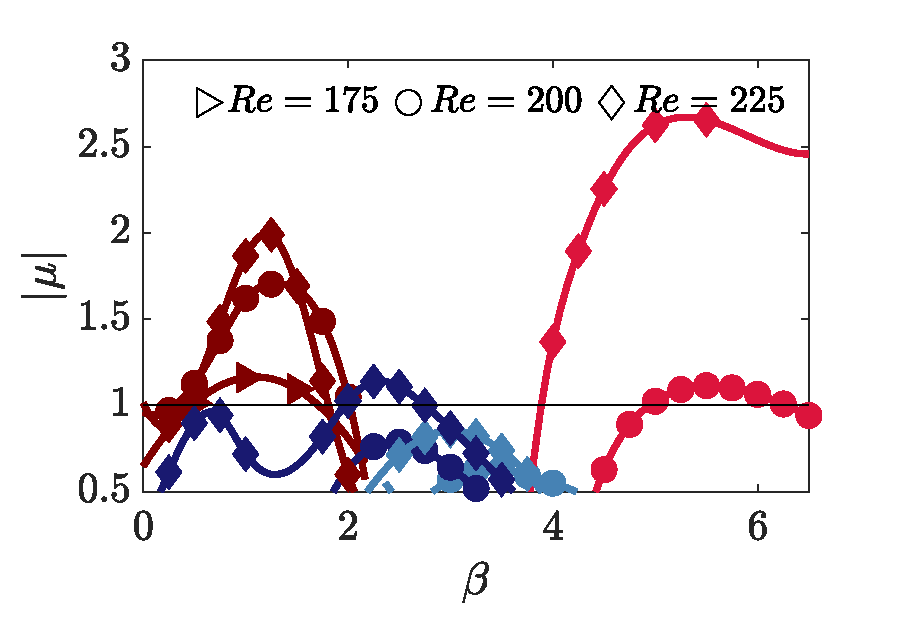
\includegraphics[width=0.49\textwidth]{./fig/AR1/neutralb.eps}
  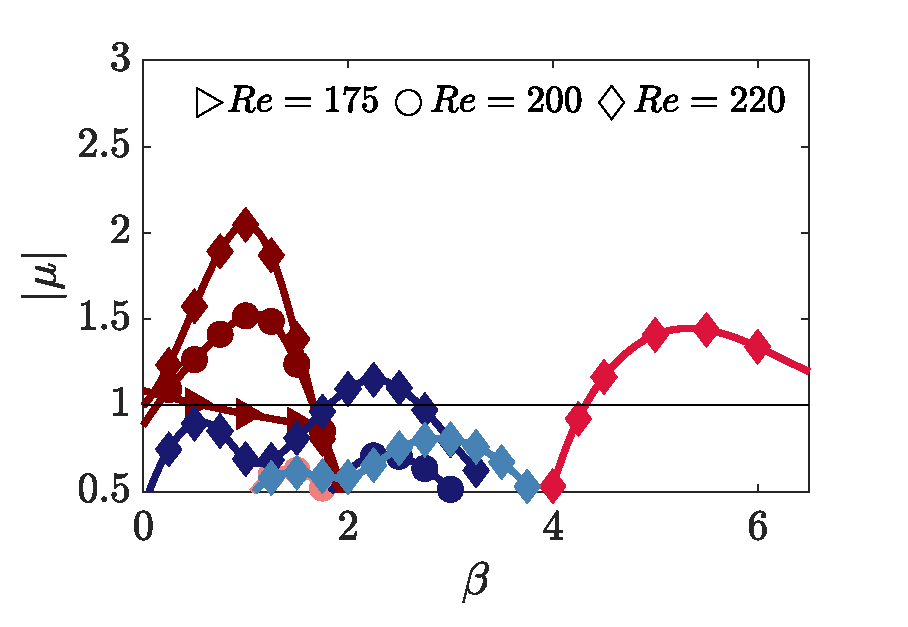
\includegraphics[width=0.49\textwidth]{./fig/AR1p25/neutralb.eps}  
  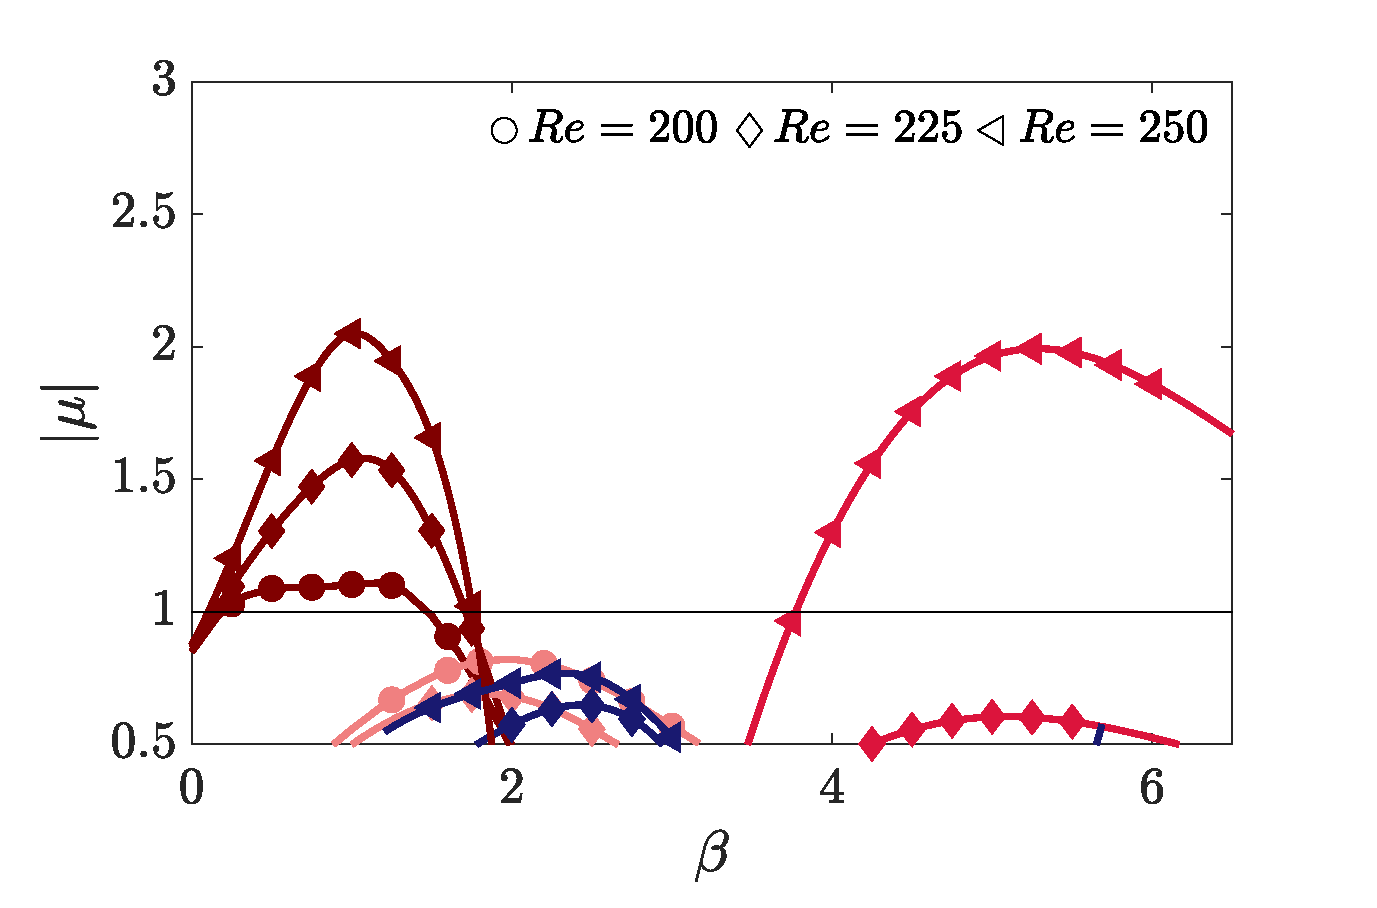
\includegraphics[width=0.49\textwidth]{./fig/AR1p5/neutralb.eps}    
  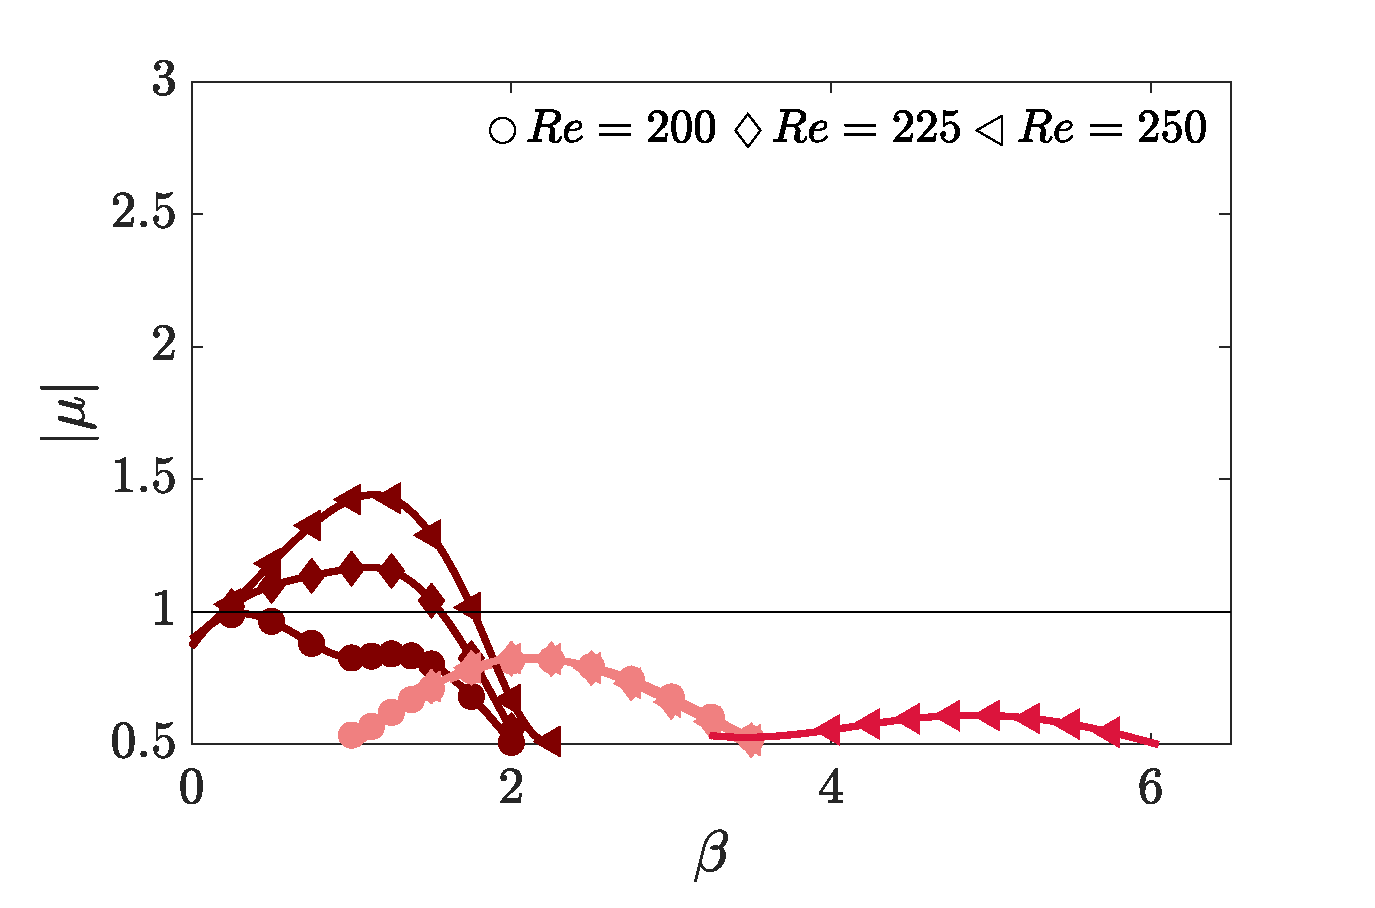
\includegraphics[width=0.49\textwidth]{./fig/AR1p75/neutralb.eps}       
  \caption{Top: multipliers for $\AR=1$, $\AR=1.25$ and $\AR=1.5$ at $Re=200$; the red line refers to mode $A$, the grey line to mode $C$, the green line to mode $B$ and the light blue line refers to mode $B'$. Mode $B'$ has the same spatio-temporal symmetry of mode $B$, but its characteristic wavelength is much smaller, being similar to that of mode $A$. This mode resembles that found for elongated bodies with elliptic leading edge by \cite{ryan-etal-2005}.}
  \label{fig:mult_AR1_AR1p75}
\end{figure}
%
\begin{figure}
  \centering
  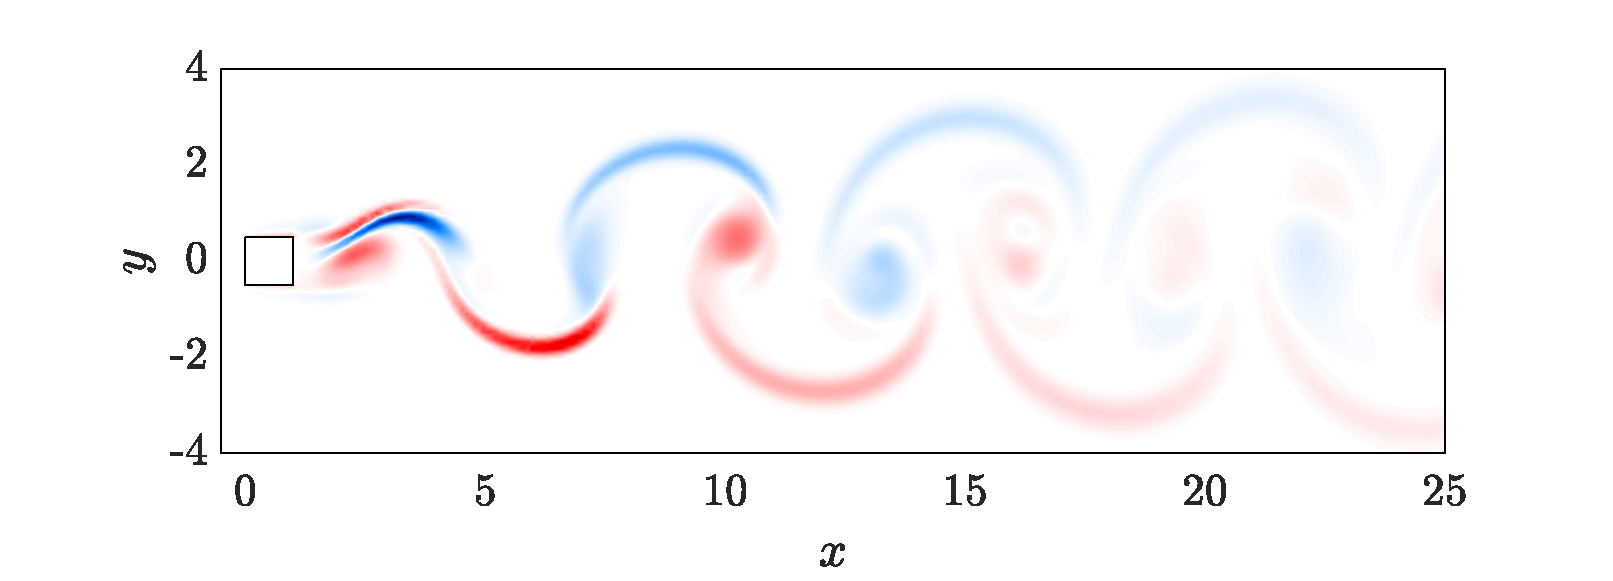
\includegraphics[width=0.49\textwidth]{./fig/AR1/omegax_Re200_beta_1p5_modeA.eps}
  \includegraphics[width=0.49\textwidth]{./fig/AR1p25/omegax_Re200_beta_5p5_modeB.eps}
  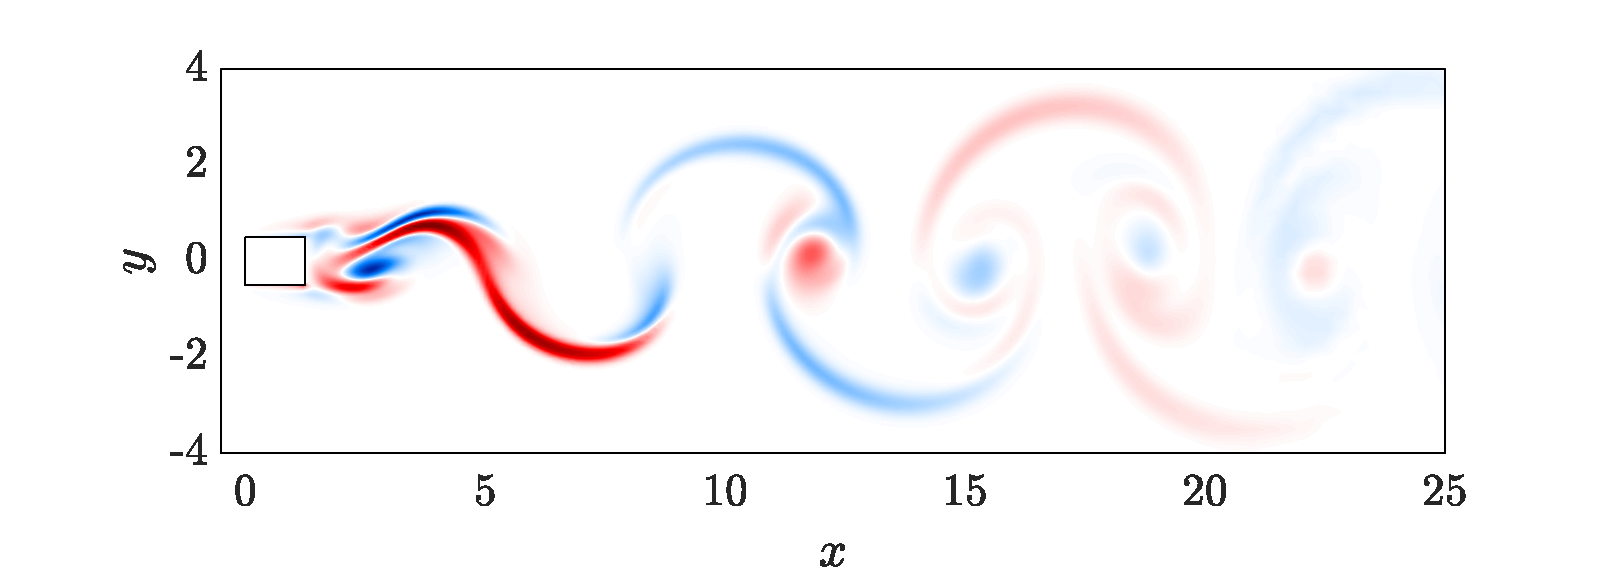
\includegraphics[width=0.49\textwidth]{./fig/AR1p25/omegax_Re230_beta_2p25_modeC.eps}
  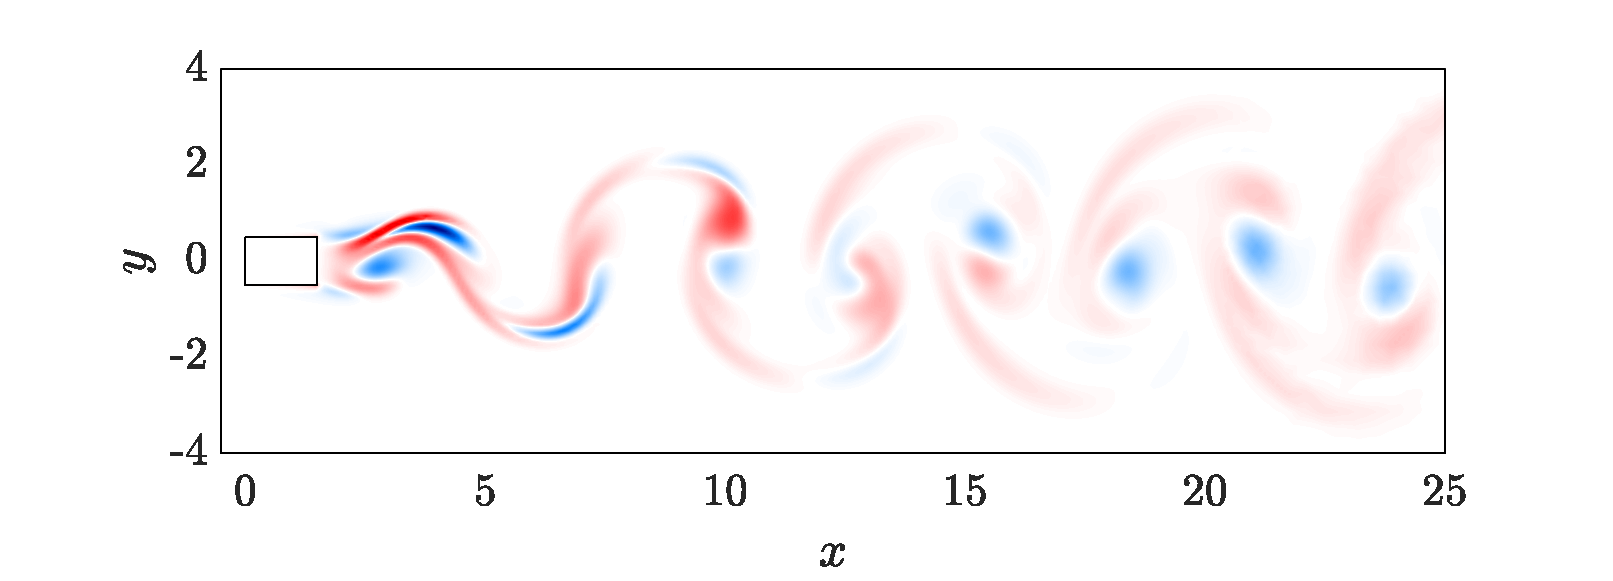
\includegraphics[width=0.49\textwidth]{./fig/AR1p5/omegax_Re200_beta_2p2_modeBp.eps}
  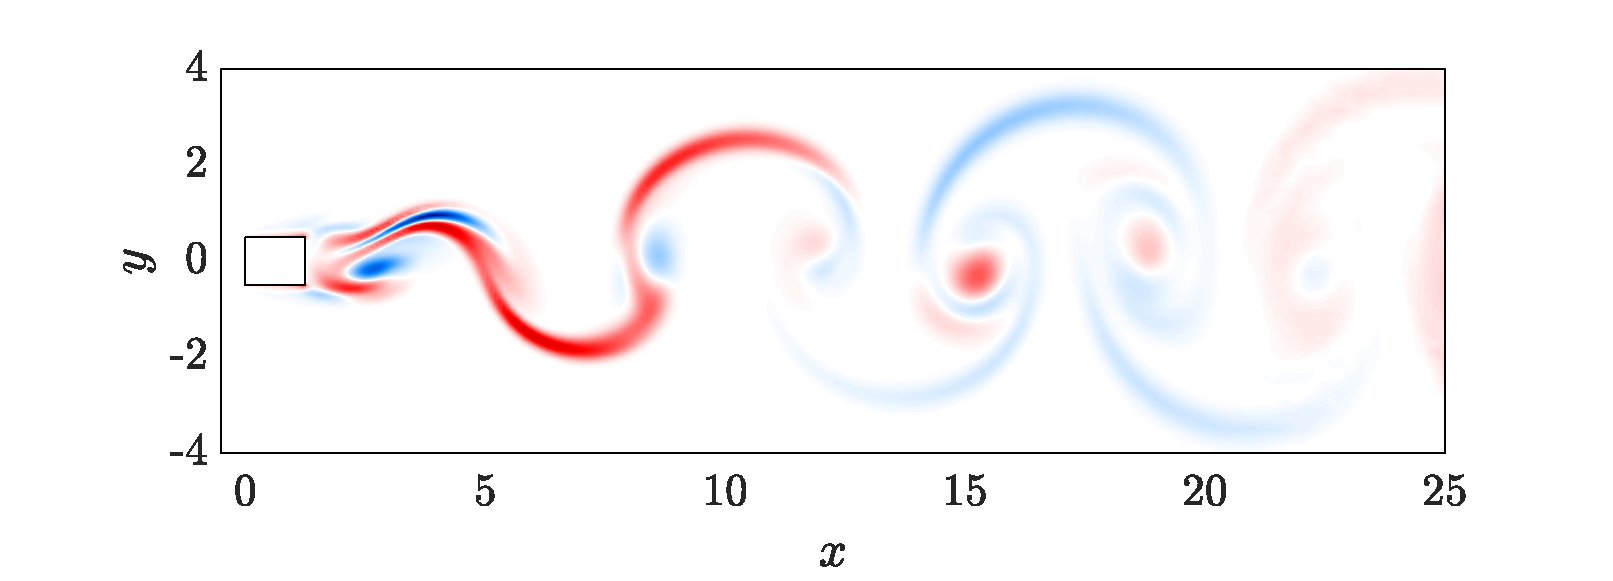
\includegraphics[width=0.49\textwidth]{./fig/AR1p25/omegax_Re230_beta_2p25_modeD.eps}
  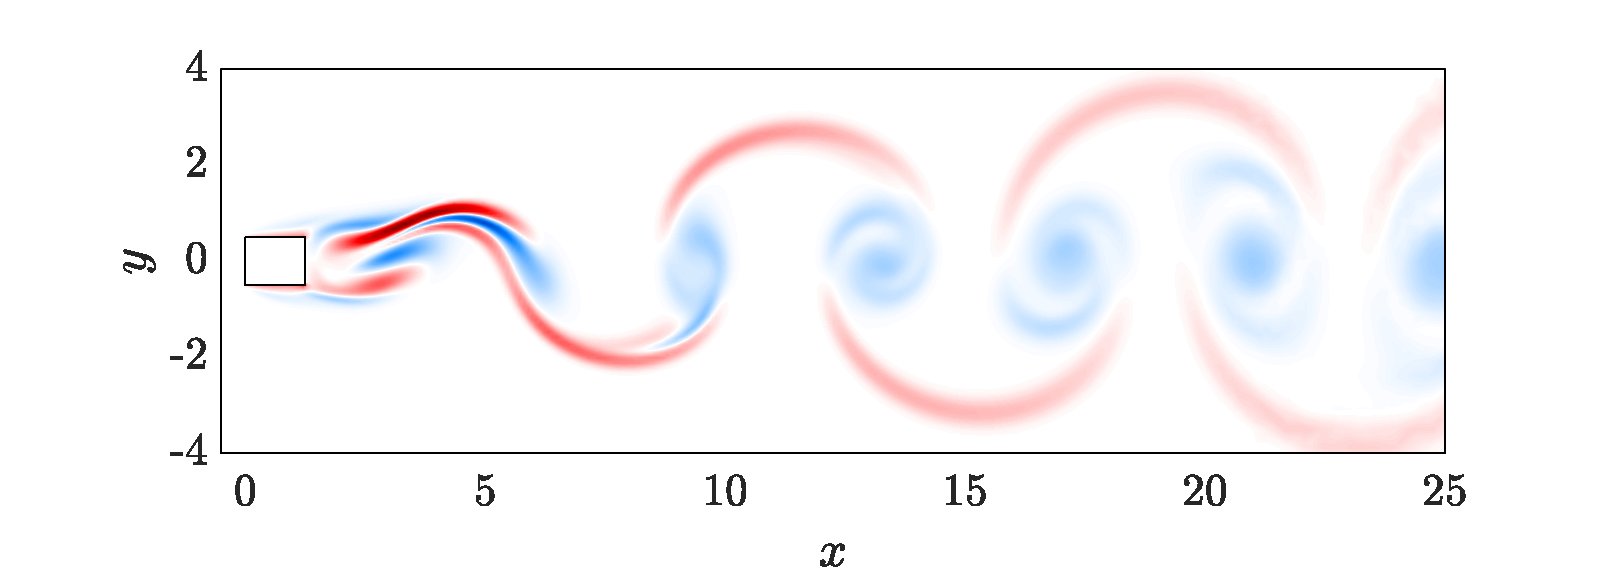
\includegraphics[width=0.49\textwidth]{./fig/AR1p25/omegax_Re240_beta_0p5_modeBpp.eps}
  \caption{Spatial structure of the modes for $1 \le AR \le 1.75$ and $175 \le Re \le 250$. Top left: mode A for $\AR=1$, $Re=200$ and $\beta=1.5$. Top right: mode B for $\AR=1.25$, $Re=200$ and $\beta=5.5$. Centre left: mode QP for $\AR=1.25$, $Re=230$ and $\beta = 2.25$. Centre right: mode $B'$ for $\AR=1.5$, $Re=200$ and $\beta=2.2$. Bottom left: mode QP' for $\AR=1.25$, $Re=230$ and $\beta=2.25$. Bottom right: mode B'' for $\AR=1.25$, $Re=240$ and $\beta=0.5$.}
  \label{fig:modes}
\end{figure}
%
As mentioned in \S\ref{sec:intro}, for $\AR=1$ three distinct modes become unstable in rapid succession. Mode A first becomes unstable at $Re \approx 175$ with a characteristic wavelength of $\lambda_A \approx 5$ ($\beta_A \approx 1.2$) and the following spatio-temporal symmetry 
%
\begin{equation}
  \hat{\omega}_x(x,y,\beta,t) = - \hat{\omega}_x(x,-y,\beta,t+/2)
\end{equation}
%
Mode B becomes unstable at $Re \approx 200$, has a characteristic wavelength $\lambda_B \approx 1$ ($\beta_B \approx 5.8$) and satisfies the symmetry:
%
\begin{equation}
  \hat{\omega}_x(x,y,\beta,t) = + \hat{\omega}_x(x,-y,\beta,t+T/2).
\end{equation}
%
Finally, mode QP becomes unstable at the higher $Re \approx 230$ with a characteristic wavelength of $\lambda_{QP} \approx 2.7$ ($\beta_{QP} \approx 2.3$). These results are in excellent agreement with our findings shown in figure~\ref{fig:mult_AR1_AR1p75}$(a)$ and \ref{fig:modes}, providing a validation of our numerical approach.

Figure~\ref{fig:mult_AR1_AR1p75}(b-d) illustrates the effect of increasing the aspect ratio. As $\AR$ increases, the onset of secondary instabilities is progressively delayes: fixing $Re$ our results show a consistent decrease inthe modulus of the Floquet multipliers associated with the three known modes, indicating a more stable base flow for longer bodies. Quantitativley, the critical Reynolds number increases from $Re_{c2} \approx 175$ for $\AR=1$ to approximately $Re_{c2} =200-225$ for $\AR=1.75$. This trend aligns with the delayed onset of the primary instability as $\AR$ increases reported by \cite{chiarini-quadrio-auteri-2021}. Despite the stabilising effect, the sequence of bifurcations remains essentially unchanged for $1 \le \AR \le 1.75$, with mode A becoming unstable first, followed by mode B. Nevertheless, for the investigated values of $Re$ mode $QP$ is not dected for $\AR>1.5$. The characteristic wavelengths of modes A and B exhibit only marginal variations with $\AR$, consistent with the findings of \cite{choi-yang-2014} for $\AR<1$. 

In addition to the three established modes, a new mode, denoted B', emerges for $\AR>1$. Mode B' shares the same spatio-temporal symmetry as mode B, but is characterised by a significantly longer wavelength, comparable to that of mode A; see figure \ref{fig:modes_AR1_AR1p75}. A mode with similar features --- both in wavelength and symmetry --- was previously reported by \cite{ryan-etal-2006} in the wake of elongated bodies with streamlined LE and blunt TE. Within the parameter range considered here, mode B' remains stable for all cases.

\begin{figure}
  \centering
  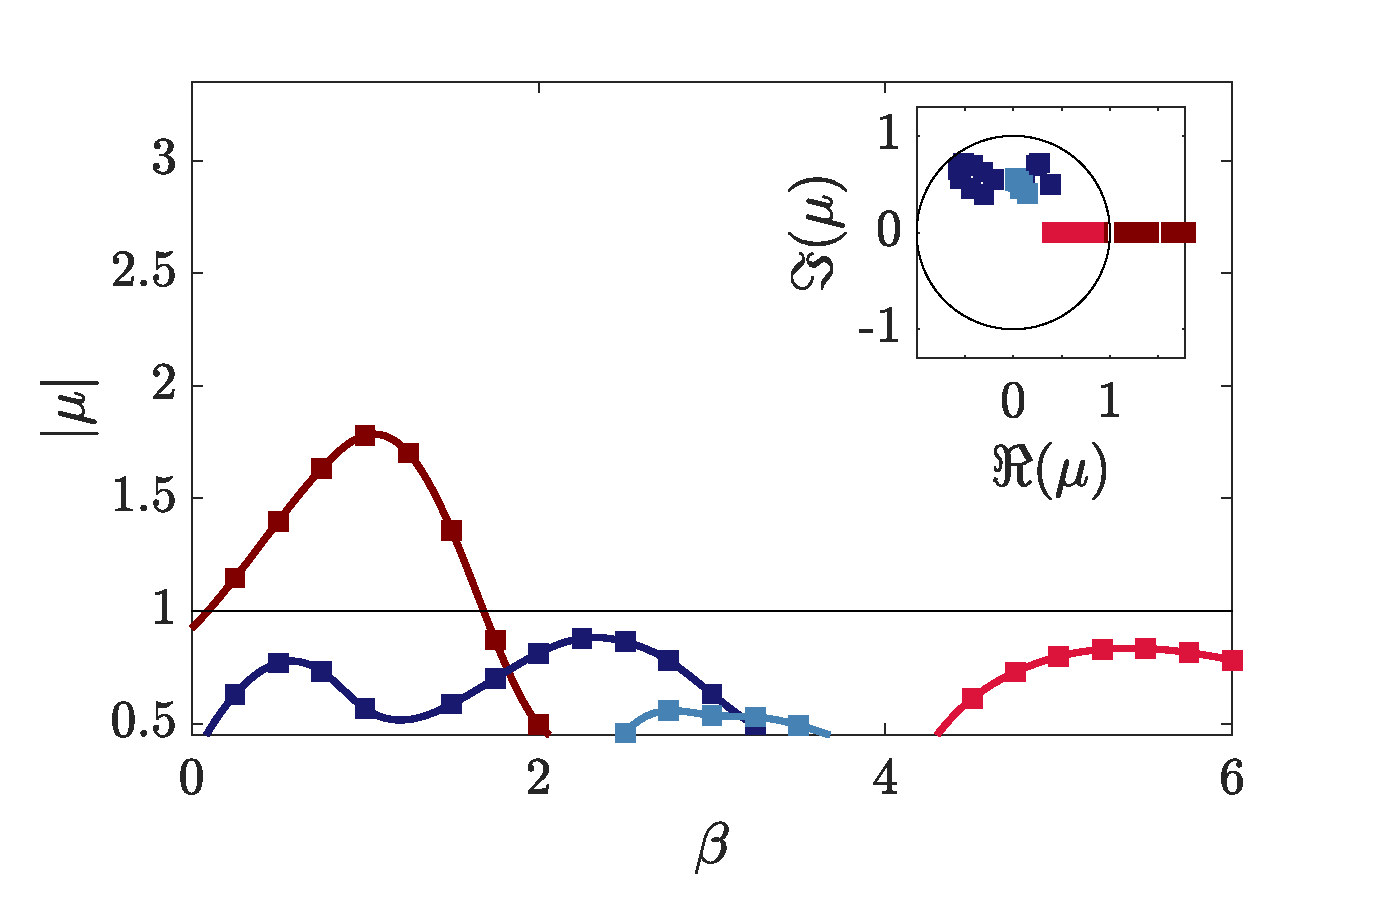
\includegraphics[width=0.49\textwidth]{./fig/AR1p25/mu_beta_Re210.eps}
  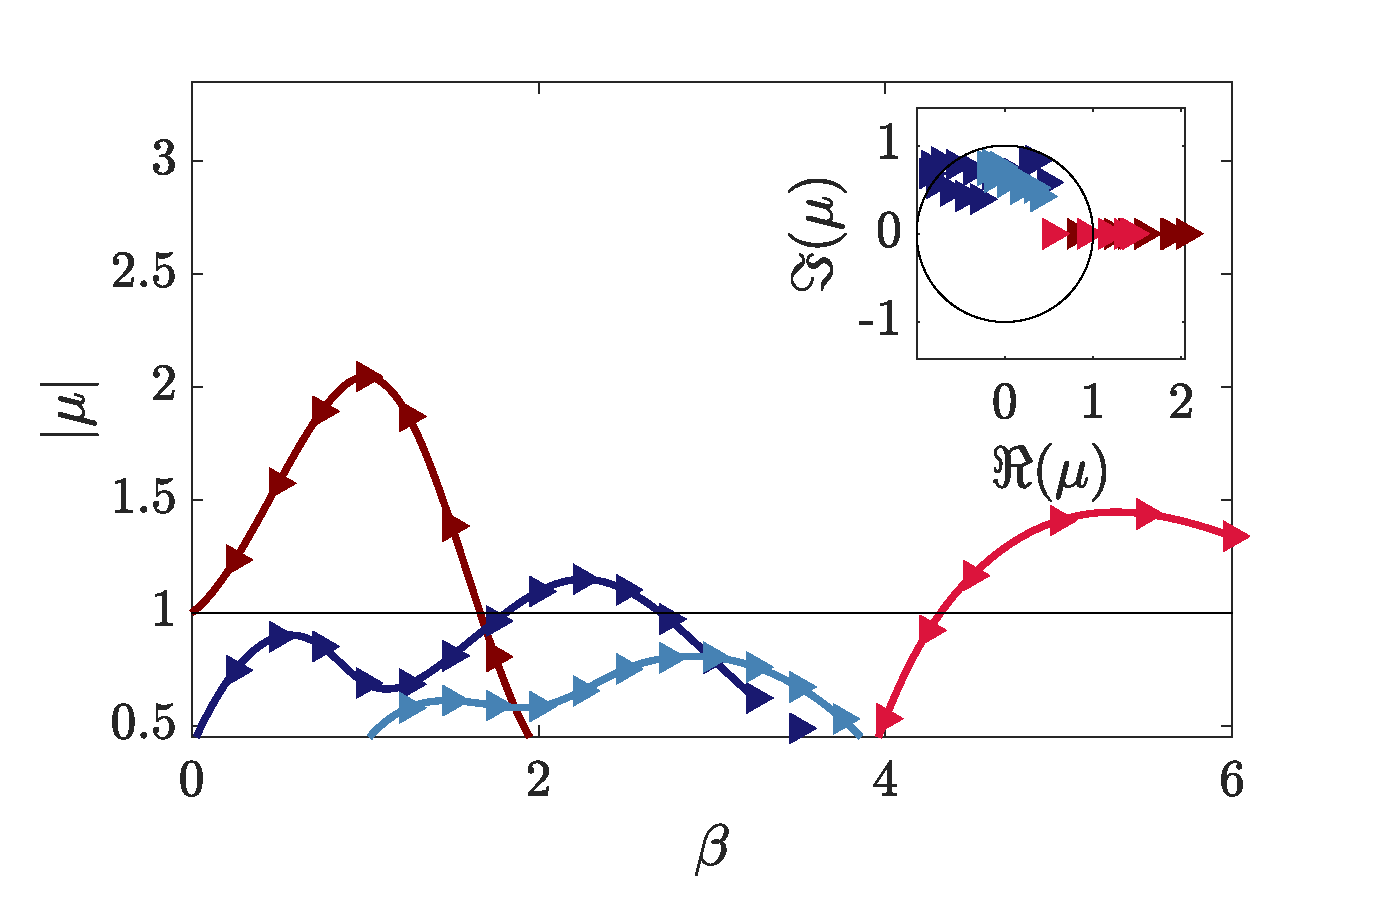
\includegraphics[width=0.49\textwidth]{./fig/AR1p25/mu_beta_Re220.eps}
  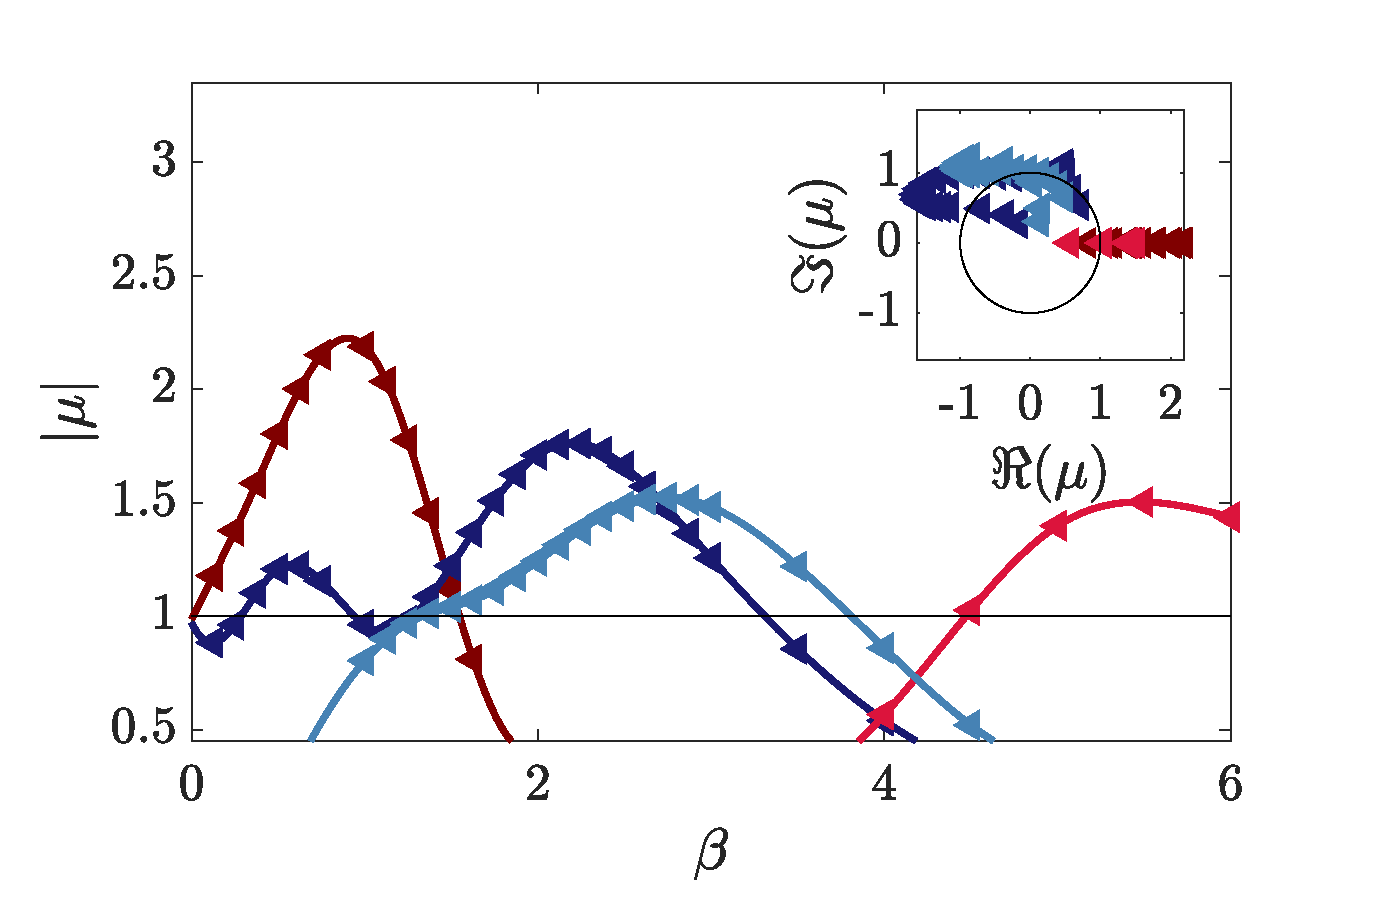
\includegraphics[width=0.49\textwidth]{./fig/AR1p25/mu_beta_Re230.eps}
  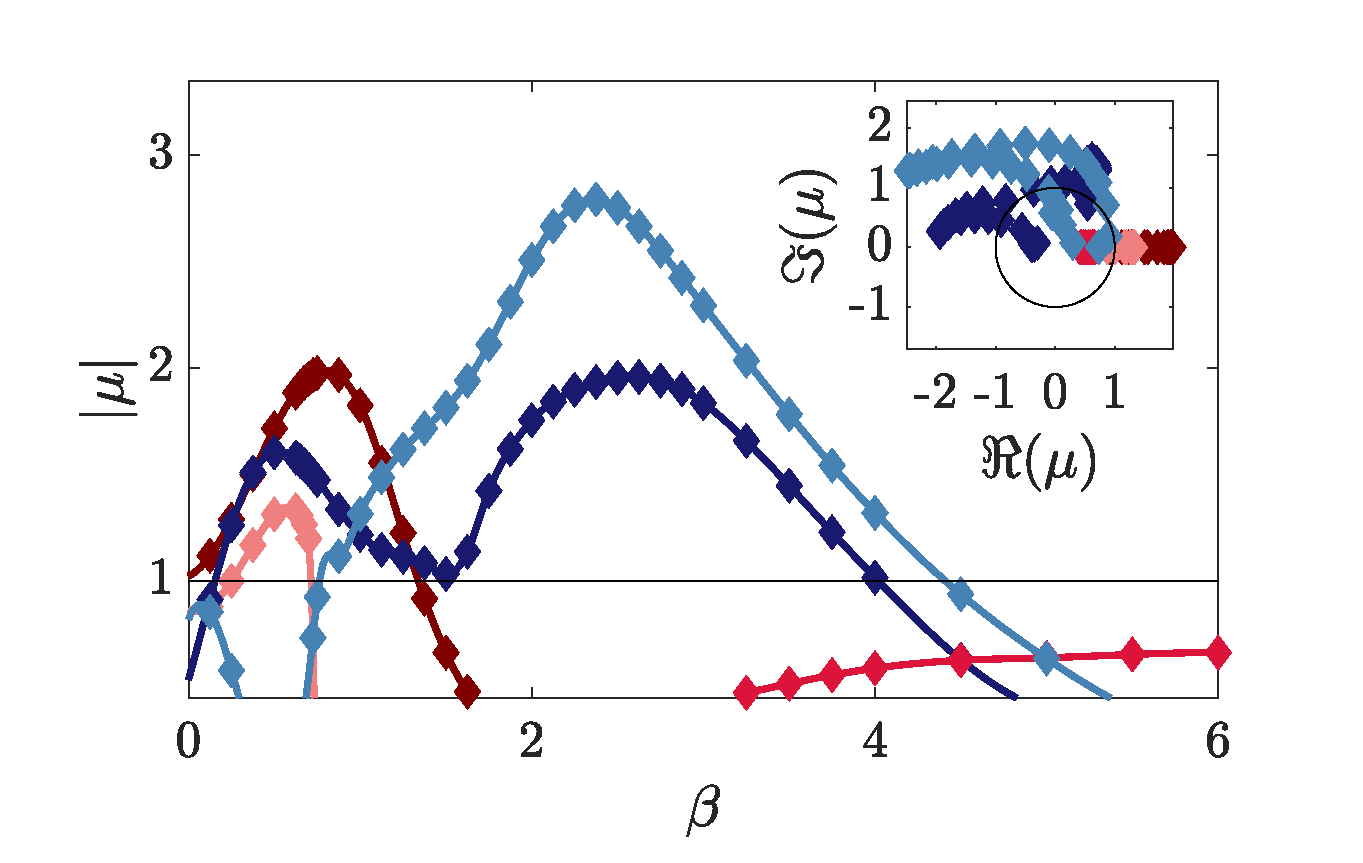
\includegraphics[width=0.49\textwidth]{./fig/AR1p25/mu_beta_Re240.eps}
  %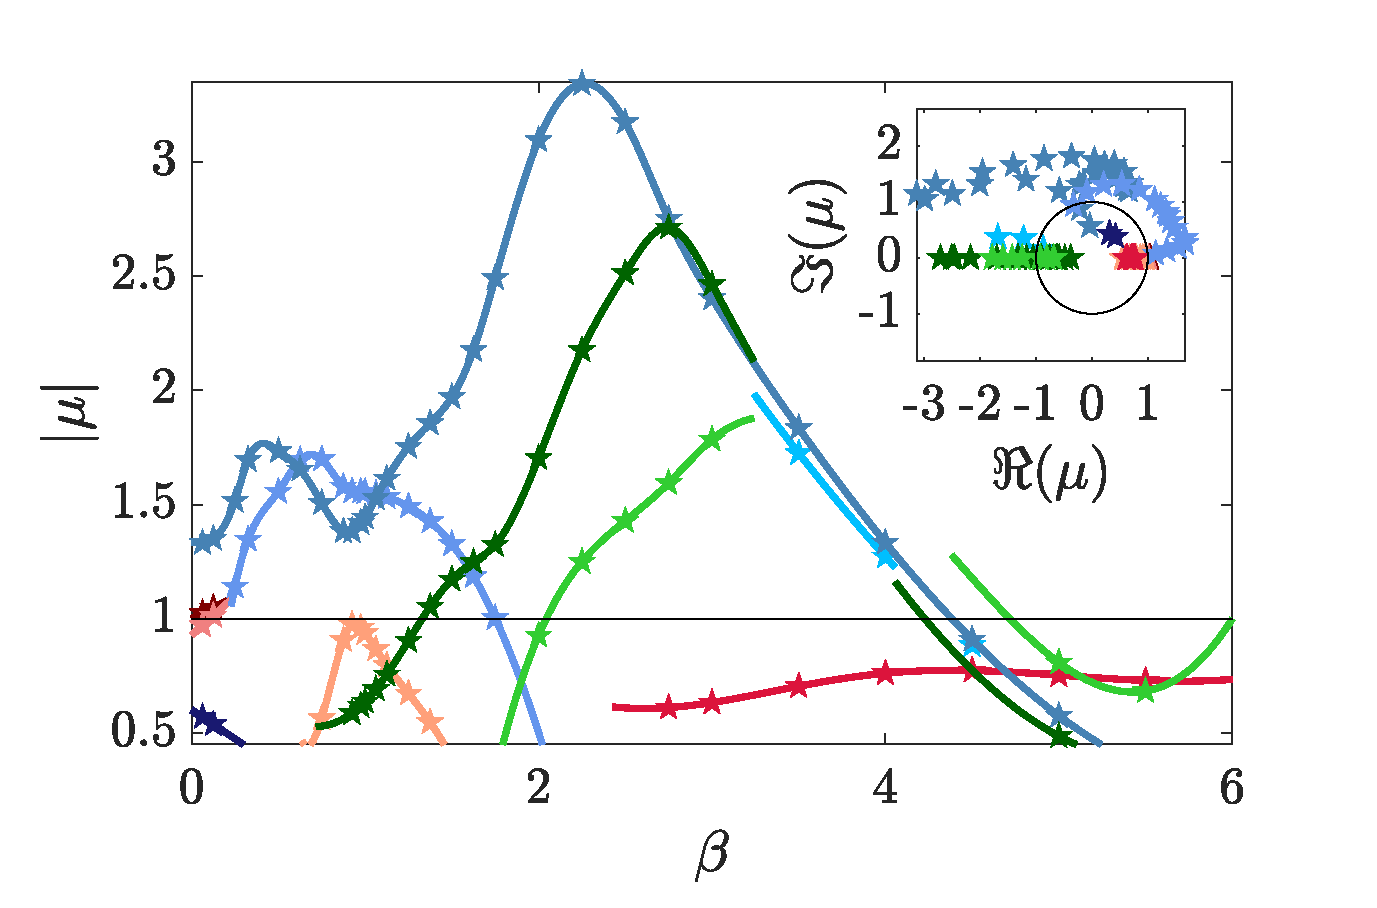
\includegraphics[width=0.49\textwidth]{./fig/AR1p25/mu_beta_Re250.eps}
  \caption{Modulus of the Floquet multipliers for $\AR=1.25$ at different $Re$. In order, the panels are for $Re=210$, $Re=220$, $Re=230$, $Re=240$ and $Re=250$.}
  \label{fig:mult-AR1p25}
\end{figure}
%
Figure \ref{fig:mult-AR1p25} details the dependence of the multipliers on $Re$ for the intermediate $\AR=1.25$ case. We observe that $\mu_A$ and $\mu_B$ have a non monotonic dependence on $Re$, meaning that modes A and B are destabilised when $Re$ increases up to $Re = 200$ and then stabilise again when further increasing it. For $Re=240$ mode B is stable. For this intermediate $\AR$ additional multipliers cross the unit circunference for $Re \ge 230$. At $Re \approx 230$ a pair of complex conjugate multipliers an additional quasi-periodic mode becomes unstable (hereafter referred as mode QP'). At $Re \approx 240$ a multiplier with positive real part crosses the unit circumference, being associated to a synchronous mode having the same symmetries as mode $B$ and $B'$, but a much shorter characteristic wavelength, i.e. $\beta \approx 0.5$. This mode is hereafter referred as mode $B'$. Figure \ref{fig:modes}(e-f) shows the spatial structure of these modes.




